%% Package and Class "uiucthesis2014" for use with LaTeX2e.
\documentclass[edeposit,fullpage]{uiucthesis2018}

\usepackage[utf8]{inputenc}
\usepackage{graphicx}
\usepackage{float}
\usepackage{amsmath}
\usepackage[version=4]{mhchem} % \ce{^{227}_{90}Th+}

\usepackage[acronym,toc]{glossaries}
\include{acros}

\usepackage{xspace}
\usepackage{graphics}
\usepackage{float} 
\newcommand{\Cycamore}{\textsc{Cycamore}\xspace}
\newcommand{\Cyclus}{\textsc{Cyclus}\xspace}


\usepackage{placeins}
\usepackage{booktabs} % nice rules (thick lines) for tables
\usepackage{microtype} % improves typography for PDF

\usepackage[hyphens]{url}
\usepackage{hyperref}
\usepackage{subfig}
\usepackage{hhline}
\usepackage{amsmath}
\usepackage{color}
\usepackage{multirow}
\usepackage{siunitx}
\sisetup{
    input-decimal-markers = .,input-ignore = {,},table-number-alignment = right,
    group-separator={,}, group-four-digits = true
}
\usepackage{fourier}
\usepackage{booktabs}
\newcommand\tab[1][1cm]{\hspace*{#1}}

\usepackage{threeparttable, tablefootnote}

%tikzpicture fit to page width
\usepackage{environ}
\makeatletter
\newsavebox{\measure@tikzpicture}
\NewEnviron{scaletikzpicturetowidth}[1]{%
  \def\tikz@width{#1}%
  \def\tikzscale{1}\begin{lrbox}{\measure@tikzpicture}%
  \BODY
  \end{lrbox}
  \pgfmathparse{#1/\wd\measure@tikzpicture}%
  \edef\tikzscale{\pgfmathresult}%
  \BODY
}

\usepackage{tabularx}
\newcolumntype{b}{>{\hsize=1.0\hsize}X}
\newcolumntype{q}{>{\hsize=0.5\hsize}X}
\newcolumntype{R}{>{\raggedleft\arraybackslash\hsize=0.5\hsize}X}
\newcolumntype{z}{>{\hsize=0.75\hsize}X}
\newcolumntype{s}{>{\hsize=.5\hsize}X}
\newcolumntype{m}{>{\hsize=.75\hsize}X}

\usepackage{cleveref}
\usepackage{datatool}
\usepackage[numbers]{natbib}
\usepackage{notoccite}


\usepackage{tikz}
\usetikzlibrary{positioning, arrows, decorations, shapes}

\usetikzlibrary{shapes.geometric,arrows}
\tikzstyle{process} = [rectangle, rounded corners, minimum width=2.5cm, minimum height=1cm,text centered, draw=black, fill=blue!30]

\tikzstyle{object} = [ellipse, rounded corners, minimum width=3cm, minimum height=1cm,text centered, draw=black, fill=green!30]
\tikzstyle{objectr} = [ellipse, rounded corners, minimum width=3cm, minimum height=1cm,text centered, draw=black, fill=red!30]

\tikzstyle{empty} =  [rectangle, rounded corners, minimum width=2.5cm, minimum height=0.7cm,text centered, draw=black, fill=white!30]
\tikzstyle{arrow} = [thick,->,>=stealth]


\title{Seifert Thesis}
\author{Luke Seifert}
\department{Nuclear, Plasma, Radiological Engineering}
%\schools{B.S., University of Illinois - Urbana Champaign, 2017}
\schools{}
\msthesis
\advisor{Madicken Munk}
%\advisor{Madicken Munk, Kathryn D. Huff}
\degreeyear{2022}
\committee{Madicken Munk \\ Tomasz Kozlowski}
%\committee{Assistant Professor Kathryn D. Huff, Adviser \\ Professor Segundo Lector }


\begin{document}
\maketitle

\frontmatter
%% Create an abstract that can also be used for the ProQuest abstract.
%% Note that ProQuest truncates their abstracts at 350 words.
%\begin{abstract}

%Abstract.

%\end{abstract}

%\chapter*{Acknowledgments}

%Acks.

%% The thesis format requires the Table of Contents to come
%% before any other major sections, all of these sections after
%% the Table of Contents must be listed therein (i.e., use \chapter,
%% not \chapter*).  Common sections to have between the Table of
%% Contents and the main text are:
%%
%% List of Tables
%% List of Figures
%% List Symbols and/or Abbreviations
%% etc.

\tableofcontents
\listoftables
\listoffigures

%% Create a List of Abbreviations. The left column
%% is 1 inch wide and left-justified
%\chapter{List of Abbreviations}
%\printglossaries
%% Create a List of Symbols. The left column
%% is 0.7 inch wide and centered

\pagebreak
\mainmatter

\chapter{Introduction}
\newcommand{\minus}{\scalebox{0.65}[1.0]{$-$}}
\renewcommand*\descriptionlabel[1]{\hspace\leftmargin$#1$}
\setcounter{tocdepth}{5}
\setcounter{secnumdepth}{5}

%\section{Energy}

%In modern society, the usefulness and convenience supplied by advancing technologies has allowed quality of life to increase drastically over time. Within these advancing technologies, ranging from air conditioning to food production, there is a common thread of energy requirement. To cool the air, energy is required in order to compress, pressurize, and cool the refrigerant. To produce food, energy is required to pump water, create fertilizer, and operate heavy machinery. Thus, the importance of energy is significant in maintaining and developing quality of life for society.

%However, energy is not free, and it takes effort to harvest and convert energy into usable forms. For wind power, this means building large turbines which can be turned by the wind. For solar power, this means building solar panels, which convert photons from the sun into electrical energy. However, for most large-scale electrical generation needs, it is more efficient for the conversion aspect to use boiling water to turn a turbine, which then generates electricity, as can be seen in Figure \ref{fig:energy-gen-methods}. Regardless of how it is generated, electricity can then be transported or stored to be used by people for any variety of purpose. 

%\begin{figure}[H]
%  \centering
%  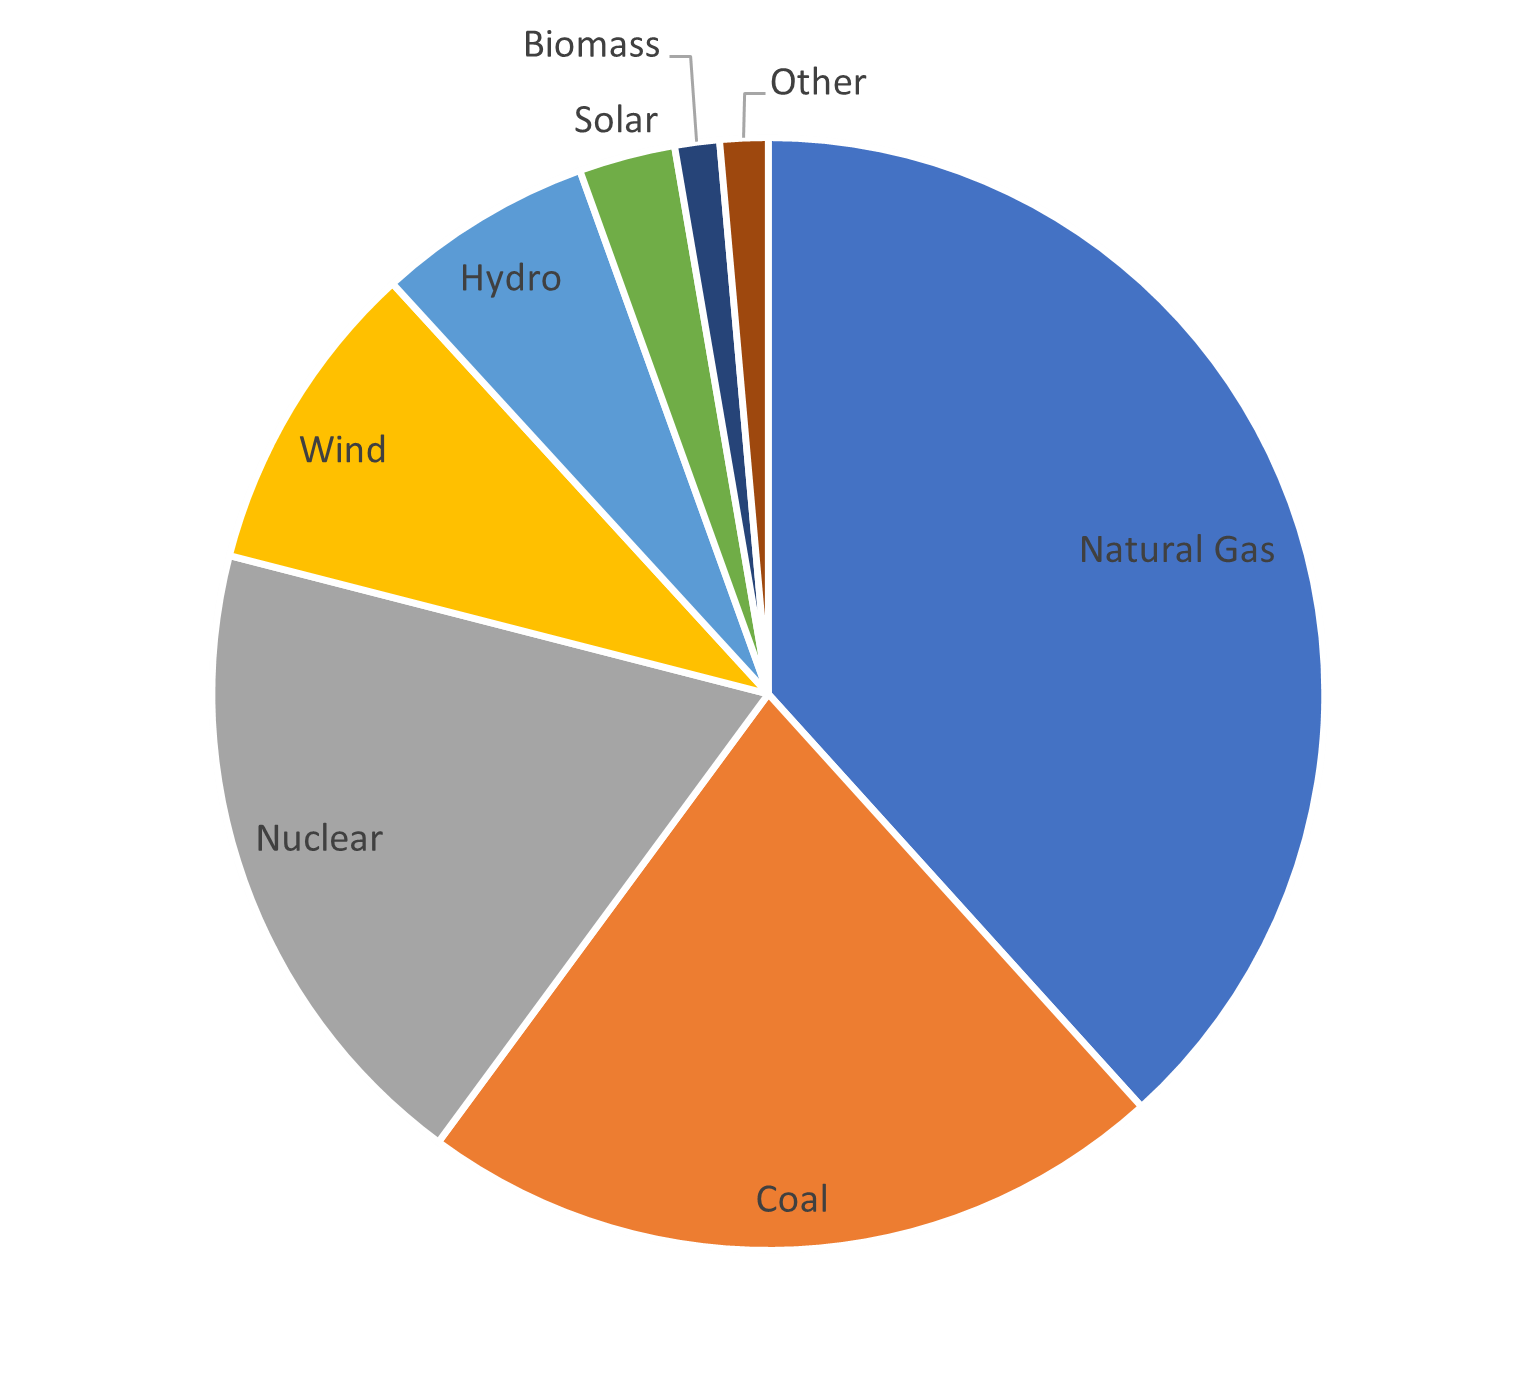
\includegraphics[scale=0.7]{images/US-energy-prod.png}
%  \caption{Energy generation in the United States in 2021 from the US %Energy Information Administration CITE %https://www.eia.gov/electricity/monthly/.}
%   \label{fig:energy-gen-methods}
%\end{figure}

%Figure \ref{fig:energy-gen-methods} shows the portion of energy generation. From this figure, it can be seen that the methods which dominate energy contribution are natural gas, coal, and nuclear. Of the various methods to generate electricity, desirable characteristics would be safety, efficiency, consistency, availability, and economics. Nuclear energy is strong in these characteristics, though there is an economic problem due to high up-front costs, which are on the order of \$10 billion for a 1GW nuclear power plant \cite{du_update_2009}. 

%\section{Nuclear Energy}

%Part of the reason nuclear energy has high up-front costs is because the nuclear industry is highly safety conscious and has many regulations in place in order to minimize risks. Although this mindset increases costs, the effort has paid dividends, which is apparent when viewing the deaths associated with different energy generation methods, shown in Table \ref{tab:death-mega} \cite{brook_why_2014}.

%\begin{table}[H]
%\renewcommand{\arraystretch}{1.25}
%\caption{Mortality rates for each energy source in deaths per billion kWh %produced (recreated from \cite{brook_why_2014}).}
%\label{tab:death-mega}
%\begin{center}
%\begin{tabular}{ | c | c | }
% \hline
% Energy Source & Mortality Rate (deaths per billion kWh)\\
% \hline
% \hline
% Coal (Global Average) & 100 \\
% Biofuel/Biomass & 24 \\
% Coal (U.S.) & 15 \\
% Oil & 36 \\
% Natural Gas & 4 \\
% Hydro (Global Average) & 1.4 \\
% Solar (Rooftop) & 0.44 \\
% Wind & 0.15 \\
% Nuclear (Global Average) & 0.04 \\
 
% \hline
%\end{tabular}
%\end{center}
%\end{table}

%Even though the up-front costs are high, nuclear power plants are licensed to operate for 40 years and can get extensions to extend that time by 10-20 years \cite{bredimas_international_2008}. This means that nuclear plants are a very long term investment. An investment at this time scale is difficult to make for a private industry though, as there is less risk when investing in cheaper plants, such as natural gas. 

%In order to address the economic issue of nuclear power plants, there are many different approaches which are implemented. One of these is to build smaller, cheaper nuclear plants which are then more affordable and are have less up-front cost. Another approach is from the regulation perspective, and involves either taxing negative externalities more harshly or subsidizing carbon-free energy sources. There is also the approach of developing new generation IV reactor designs \cite{kelly_generation_2014}.

% Why MSRs, why depletion

\section{Molten Salt Reactors}

One of the generation IV reactor designs is the molten salt reactor, or MSR \cite{kelly_generation_2014}. The MSR potentially offers a lower "n'th-of-a-kind" cost of electricity when compared to coal and pressurized water reactors, which are a large portion of the nuclear fleet \cite{moir_cost_2002}. 
%Of particular interest in this thesis is the liquid fueled MSR design, which is significantly different from the current light water reactor, or LWR, designs which dominate the nuclear fleet currently in use.
%Light water reactors include boiling water reactors (BWRs) and pressurized water reactors (PWRs), both of which are well understood reactor designs currently implemented.
Light water reactors use a solid fuel containing uranium-235 with a water coolant, which also serves as a moderator to slow down the neutrons to thermal energies. This fuel generates heat as the fissile uranium-235 fissions. After some lengthy amount of depletion, it can be reshuffled or removed from the reactor to be placed into a cooling pool.

Liquid fueled molten salt reactors, instead of a solid fuel, use a liquid fuel composed of a molten salt mixed with some fissile isotope, such as uranium-235. Some of the benefits of MSRs include higher operating temperature, lower operating pressure, and high thermal conductivity and capacity of the salts. Other benefits include a high coefficiency of thermal expansion for negative temerature coefficient of reactivity, better resource utilization through higher burn-up, reduced cost of fabricating and transporting fuel elements, and the removal of fission products to improve the neutron economy \cite{serp_molten_2014}.
% WHy MSRs? How will it help nuclear? Reactivity/power density?

Using a liquid fuel allows for online reprocessing, a continuous process which can involve adding fresh fuel to the system as well as chemically removing undesirable products which are generated through fission. The system also allows for batchwise reprocessing, which is a process which occurs in discrete steps, such as salt disposal. Typically, most reprocessing involved in an MSR is continuously performed while the reactor is online.

The usefulness of reprocessing, particularly online reprocessing, is that the reactor does not need excess reactivity in order to continue operating for a long period of time. In a typical LWR, burnable poisons and control rods are used to lower reactivity at the beginning of the core life so the reactor can remain at a safe criticality over the core life. In a liquid fueled MSR, the parasitic absorbers, such as xenon-135, can be removed from the reactor. Additionally, fresh fuel salt can be added to the reactor in order to maintain stable operation.

This fresh fuel feed can include fissile isotopes, such as uranium-233 or uranium-235, fertile isotopes, such as uranium-238 or thorium-232, or some combination of both. Adding a fissile isotope to the reactor will allow for the reactor to continue fission when the isotope is fissioned by a neutron. For the fertile isotopes, the neutron must first be absorbed and the product decays, leading to a fissile isotope. This process can be seen in Equation \eqref{eq:th-pa-chain}, which is the breeding process used in the Molten Salt Breeder Reactor.

\begin{equation} \hfill
\ce{^{232}_{90}Th} + \ce{^{1}_{0}n} \longrightarrow \ce{^{233}_{90}Th} \longrightarrow \ce{^{233}_{91}Pa} \longrightarrow \ce{^{233}_{92}U}
\hfill\label{eq:th-pa-chain} \end{equation}

The half life of thorium-233 via beta decay is on the order of tens of minutes, while the half life of protactinium-233 via beta decay is roughly 27 days. Without reprocessing, the protactinium-233 remaining in the core for such a period of time would be more likely to interact with neutrons, impacting the breeding efficiency. The Molten Salt Breeder Reactor continuously chemically extracts the protactinium from the fuel salt, allowing it to decay in a separate tank. While it decays, another continuous chemical process strips uranium which is formed and brings the uranium back into the reactor, continuing the process.

\section{Depletion and Reprocessing Methods}

For molten salt reactor reprocessing, the two different physical approaches are continuous and batchwise. Additionally, these reprocessing schemes can be online, while the reactor is operating, or offline, when the reactor is shutdown. Of particular importance for MSR behaviour is online reprocessing, which changes the fuel composition while the reactor is operating.

An important type of model to simulate for reactor analysis is a depletion model, where the reactor operates for some length of time using discrete depletion steps. This model is important to determine fuel utilization, neutronic parameters at different stages in the reactor life, and to make further decisions about the reactor.

In a depletion simulation, general data is generated about the model at each depletion time step. After each of these steps, updated data is then used for the next depletion step. This updated data includes cross section data, energy spectra, neutron flux, and can include changes to temperature, volume, densities, or compositions. For MSRs, these updated changes after each depletion step need to account for the effects of online reprocessing.

In order to model online reprocessing in a depletion simulation, there are two different computational methods which can be implemented. These methods are named continuous and batchwise reprocessing methods, the same naming convention as the physical processes which they represent. However, it is fairly common for MSR analysis works which implement a phyiscally continuous reprocessing scheme to simulate this scheme using batchwise mathematical models.

Thus, this work seeks to investigate the continuous and batchwise computational reprocessing methods. This investigation involves effects of depletion step size, validity of batchwise methods approximating continuous methods, and different sub-methods within both batchwise and continuous methods which can be implemented.



\chapter{Literature Review}
\renewcommand*\descriptionlabel[1]{\hspace\leftmargin$#1$}
\setcounter{tocdepth}{5}
\setcounter{secnumdepth}{5}
\newcommand{\minus}{\scalebox{0.65}[1.0]{$-$}}

\section{Molten Salt Reactors}

Modeling and simulation of liquid fueled molten salt reactors (MSRs) differs from solid fueled reactors in two main areas. The first is in the fresh fuel feed and fission product removal streams used during operation in MSRs, called online reprocessing. Modeling an MSR without online reprocessing will cause very different results during depletion calculations due to the lack of fresh fuel and buildup of fission products. In order to simulate this reprocessing functionality, software can either use batchwise reprocessing or continuous reprocessing.

The second difference is in the movement of the fuel salt, which causes delayed neutron precursors (DNPs) to move in the core. Because the DNPs have different decay times before the delayed neutrons are born, the effect of the fuel movement on each group varies. However, the overall result is more delayed neutrons in less important regions, such as external piping, which means there is a reduced effective delayed neutron fraction in the core.
%Modeling and simulation of liquid fueled molten salt reactors (MSRs) is different from modeling and simulation of solid fueled reactors in a few different areas. Two main areas of particular importance are the online reprocessing functionality and the movement of the fuel through the reactor. The online reprocessing functionality involves removing fission products from the fuel and adding fresh fuel during operation. The movement of the fuel causes a shift in the location of delayed neutron precursors (DNPs). In solid fueled reactors, the distribution of DNPs follows the flux profile, while in MSRs the DNPs move along with the fuel. This results in a reduction in the effective delayed neutron fraction due to decay of DNPs in less important regions.

\subsection{Online Reprocessing}

The online reprocessing functionality of MSRs is simulated in different ways depending on the particular software used, and depending on the methods employed by that software. The two main ways to approach the online reprocessing problem is by either using batch-wise reprocessing or continuous reprocessing. For these approaches, the physical process may represent either approach, such as continuously removing protactinium from the core, but adding in the uranium it decays into only after some time has elapsed. Typically, however, a purely batchwise modeling approach will not fit the reprocessing design used by a reactor since online reprocessing is carried out continuously. An MSR using offline reprocessing, however, can be accurately represented using purely batchwise reprocessing.

%Codes implement batchwise reprocessing by running the simulation, stopping, and then adding and removing materials. The process is then iterated. This method is useful in that it is fairly straightforward to implement, can be calibrated to different removal efficiencies, and makes mass balancing of the core straightforward. Some issues with the batchwise approach are that using large time steps will make the results more inaccurate, it has increased computational cost with smaller time steps, and it is an approximation of the actual physical process of reprocessing. It is an approximation because, in online reprocessing of a reactor, the fission products are continuously removed while any feed flows are continuously fed into the reactor.
Codes such as SaltProc and older versions of ChemTriton implement batchwise reprocessing by running the simulation, stopping, and then adding and removing materials \cite{rykhlevskii_modeling_2019, betzler_molten_2017}. The process is then iterated. This method is useful because it is fairly straightforward to implement, easy to customize, and makes mass balancing of the core straightforward. Some issues with the batchwise approach are that using large time steps will make the results more inaccurate, it has increased computational cost with smaller time steps, it has to rerun each time step for pre-reprocessing and post-reprocessing, and it is an approximation of the actual physical process of reprocessing. It is an approximation because, in online reprocessing of a reactor, the fission products are continuously removed while any feed flows are continuously fed into the reactor.

%Continuous reprocessing is implemented by adding terms to the Bateman equation similar to an extra decay term. The benefits of using continuous reprocessing are that the model is physically accurate, it doesn't impact computational cost as much as a batchwise process, and it allows for large time steps to be used. A note should be made, however, that the time step size is still limited since the simulation will need to update based on the new material composition and evolving neutron spectrum. However, there is less error from inaccurate material removal and addition. The main downside of the continuous removal approach is that it is more cumbersome to implement and configure due to the nature of how it operates.
Codes such as Serpent2 and newer versions of ChemTriton implement continuous reprocessing by adding terms to the Bateman equation similar to an extra decay term, as can be seen in Equation (\ref{eq:Bateman_type_one_decay}) \cite{aufiero_extended_2013, jr_vicente_valdez_modeling_2020}. The benefits of using continuous reprocessing are that the model is more physically accurate, it doesn't impact computational cost as much as a batchwise process, and it allows for larger time steps to be used. However, the maximum time step size cannot become too large, or the simulation will become less accurate. This is because the neutron spectrum and cross section data does not update to the new material compositions until a new depletion step begins. 
%The main downsides of the continuous reprocessing approach are that it is more cumbersome to implement and difficult to configure due to the nature of how it operates.

Another aspect of online reprocessing that must be considered is mass balancing. For batchwise reprocessing, mass balancing can be solved in several different ways. One method is to have the net mass of the feed rate over some depletion step be equivalent to the mass removed over that same depletion step, which is the current approach used by SaltProc \cite{rykhlevskii_modeling_2019}. Alternatively, the volume of the system can be adjusted so that constant density is maintained in order to keep cross section data consistent \cite{ridley_method_2017}. Another approach is to move excess fuel salt into a bleed-off tank \cite{ridley_method_2017}. For continuous reprocessing, the depletion time steps can be much larger. This means that during the interval between steps, the mass will not be balanced. However, the same batchwise methods can be used with continuous reprocessing at new depletion steps. Implementing these approaches increases computational cost when performed in Serpent2. This is because using a single input script with depletion steps will cause each depeletion step to be run once, but altering the input script by changing volumes or removing mass to a bleed-off tank will cause the time step to be run twice.

\subsubsection{Batchwise Reprocessing}

%Imagine a process exists in which $X$\% of some element is removed from the fuel salt in the system over some time period T. For a batchwise approach, a straightforward approach would be to run the system, deplete for some time step $\tau$, remove $\gamma$\%, and repeat. The scaling term $\gamma$ for the removal efficiency is a linear approximation of the removal efficiency based on the time step adjustment and can be seen in Equation \ref{eq:batchwise_rem_eff}. An alternative approach is to establish a depletion time step $\tau$ such that the efficiency based time value $T$ is a multiple of $\tau$ and only have the batchwise removal occur at the steps when $\tau$ is a multiple of $T$. 

%\begin{equation} \hfill 
%\gamma = X \frac{\tau}{T}
%\hfill\label{eq:batchwise_rem_eff} \end{equation}
Batchwise reprocessing starts with some removal rate where $X$\% of some element is removed from the fuel salt in the system over some time period T. Over a depletion step $\tau$, $\gamma$\% of the element's mass is removed, where $\gamma$ corresponds to $X$ according to Equation (\ref{eq:batchwise_rem_eff}). The scaling term $\gamma$ for the removal efficiency is a linear approximation based on the time step adjustment in Equation (\ref{eq:batchwise_rem_eff}). If the time step used causes the removal fraction to be greater than 1, the amount removed remains at 100\% so as to not have negative mass.

An alternative approach is to establish a depletion time step $\tau$ such that the efficiency based time value $T$ is a multiple of $\tau$ and only have the $X\%$ batchwise removal occur at the steps when $\tau$ is a multiple of $T$, thus removing the need for scaling.

\begin{equation} \hfill 
\gamma = X \frac{\tau}{T}
\hfill\label{eq:batchwise_rem_eff} \end{equation}

For the Molten Salt Breeder Reactor (MSBR), SaltProc performs batchwise reprocessing every 3 days using a linear approximation of the cycle times given by Robertson et al in the ORNL report \cite{robertson_conceptual_1971, rykhlevskii_modeling_2019}. The xenon and krypton removals in SaltProc use a gas separation system equation, while the protactinium uses a modeled liquid-liquid reductive extraction process. These efficiencies differ from the cycle time values, causing slight differences in those terms. The MSBR also has two varying feed inputs of \ce{^{232}Th} and \ce{^{233}U}.

Examples of the batchwise method used in SaltProc can be seen in Equations \eqref{eq:SP_20s} and \eqref{eq:SP_60d}. Both examples show what the resulting mass removal per step, or $\gamma$, term should be for different cycle time values. The first shows a cycle time of 20s, which is shorter than the step time of 3 days. This results in a removal rate over 100\%, which is set to 100\%. The second shows a cycle time of 60 days, longer than the step size. This results in a 5\% removal per step. An alternative approach to the second example, which is implemented in the earlier versions of SaltProc, is to perform no removal until 60 days have elapsed and then remove 100\% of material.

\begin{equation} \hfill
X = 100\%, T = 20 s, \tau = 3 d \rightarrow \gamma > 100\% \rightarrow 100\% 
\hfill\label{eq:SP_20s} \end{equation}

\begin{equation} \hfill
X = 100\%, T = 60 d, \tau = 3 d \rightarrow \gamma = 5\%
\hfill\label{eq:SP_60d} \end{equation}

\subsubsection{Continuous Reprocessing}

%For a continuous approach, removing some fraction is dependent upon the particular isotope since the approach involves adding a term to the Bateman equation. This is one of the methods used in Serpent2 continuous reprocessing, where separations are only performed based on the element, not each particular isotope, an extension developed by Aufiero et al \cite{aufiero_extended_2013}. Equation \ref{eq:Bateman_default} shows the generic form of the Bateman equation, while Equation \ref{eq:Bateman_type_one_decay} shows the terms added to Equation \ref{eq:Bateman_default}, which are the reprocessing constants, or $\lambda_{r}$ added. 
The continuous approach manipulates the Bateman equation by adding a reprocessing term, which contains a reprocessing constant and the concentration of the isotope. This is one of the methods used in Serpent2 continuous reprocessing, an extension developed by Aufiero et al \cite{aufiero_extended_2013}. Equation (\ref{eq:Bateman_default}) shows the generic form of the Bateman equation, while Equation (\ref{eq:Bateman_type_one_decay}) shows the terms added to Equation (\ref{eq:Bateman_default}), which are the reprocessing constants, $\lambda_{r}$. These terms represent removal of the current isotope as well as feed of the current isotope from other sources.

\begin{equation} \hfill
\begin{split}
%\frac{dN}{dt} = \sum_j \lambda_j N_j + \gamma \Sigma_f \phi + \Sigma_k \phi - \lambda N - \Sigma \phi - C
\frac{dN_j}{dt}_{base} = \sum_{i \neq j}  & \left [ \left( \gamma_{i \rightarrow j} \sigma_{f, i} \Phi + \lambda _{i \rightarrow j} + \sigma_{i \rightarrow j} \Phi \right) N_i \right ]\\
 & - \left ( \lambda_j + \sigma_j \Phi \right ) N_j
\end{split}
\hfill\label{eq:Bateman_default} \end{equation}

\begin{equation} \hfill
%\frac{dN}{dt} = \sum_j \lambda_j N_j + \gamma \Sigma_f \phi + \Sigma_k \phi - \lambda N - \Sigma \phi - C
%\frac{dN_j}{dt} = \sum_{i \neq j} \left [ \left( \gamma_{i \rightarrow j} \sigma_{f, i} \Phi + \lambda _{i \rightarrow j} + \lambda _{reproc, i \rightarrow j} + \sigma_{i \rightarrow j} \Phi \right) N_i \right ] - \left ( \lambda_j + \lambda_{reproc, j} + \sigma_j \Phi \right ) N_j
%\frac{dN_j}{dt} = \sum_{i \neq j} \left [ \left( \gamma_{i \rightarrow j} \sigma_{f, i} \Phi + \lambda _{i \rightarrow j} + \lambda _{r, i \rightarrow j} + \sigma_{i \rightarrow j} \Phi \right) N_i \right ] - \left ( \lambda_j + \lambda_{r, j} + \sigma_j \Phi \right ) N_j + \sum_{mat} \lambda _{r, i \rightarrow j} N_i
\frac{dN_j}{dt}_{net} = \frac{dN_j}{dt}_{base} -  \lambda_{r, j} N_j + \sum_{mat} \lambda _{r, i \rightarrow j} N_i
\hfill\label{eq:Bateman_type_one_decay} \end{equation}

The symbols given in the equations are defined as follows from Equation \cite{leppanen_development_2007}:
\begin{description}
\item[N_j] is the atomic density of isotope j.
\item[\gamma_{i \rightarrow j}] is the fractional fission product yield of $j$ in the fission of isotope $i$.
\item[\sigma_{f, i}] is the microscopic fission cross section of isotope $i$.
\item[\Phi] is the spectrum-averaged scalar flux in the fuel region.
\item[\lambda _{i \rightarrow j}] is the decay constant of decay $i \rightarrow j$.
%\item[\lambda _{r, i \rightarrow j}] is the reprocessing constant for feed of $i \rightarrow j$ 
\item[\sigma_{i \rightarrow j}] is the microscopic transmution cross section of reaction $i \rightarrow j$.
\item[N_i] is the atomic density of isotope $i$.
\item[\lambda_j] is the decay constant of isotope $j$.
\item[\lambda_{r, j}] is the reprocessing constant for removal of isotope $j$.
\item[\sigma_j] is the microscopic total transmutation cross section of isotope $j$.
\item[\lambda _{r, i \rightarrow j}] is the reprocessing constant for feed of material $i \rightarrow j$.
\end{description}

%It can be seen visually that the reprocessing removal essentially operates as increasing the decay rate when applied in this manner. For example, increasing the decay rate of a particular element in a given material in Serpent2 also requires another material to gain a feed rate equivalent to that decay rate. The feed rate of a particular material is given by summing the removal rates of other materials for each isotope.
Equation \eqref{eq:Bateman_type_one_decay} shows that the reprocessing removal has the same mathematical operation as the decay rate. Unlike decay, the isotopes removed by reprocessing instead are transfered to a different material, which operates as a feed for that material. This can be seen in the summation term, which sums over the different materials and moves them from material $i$ to material $j$.

Serpent2 has three different settings for continuous reprocessing which alter the effect on the Bateman equations. The zeroth setting does not conserve mass, so it will not be discussed. The first setting, which adds a decay-like term to the Bateman equation, is shown in Equations (\ref{eq:Bateman_default}) and (\ref{eq:Bateman_type_one_decay}). This approach of adding a decay-like term to the Bateman equation has been done with other codes \cite{jr_vicente_valdez_modeling_2020, rodriguez-vieitez_transmutation_2002}. For this setting, three different approaches are implemented in order to compare their results.


The first approach is labeled the Cycle Time Decay (CTD) approach. It takes half the value of the cycle times and treats them as half life values. A similar method of treating removal periods for reprocessing can be seen in Brovchenko et al \cite{brovchenko_neutronic_2019}. Equation (\ref{eq:CTDex}) shows how this approach works with a cycle time of 20 seconds. The operation cuts the cycle time in half and then calculates the decay constant, or reprocessing constant, using the half life from the cycle time.

\begin{equation} \hfill
20s \rightarrow \tau = 10s \rightarrow \lambda_{r} = \frac{ln(2)}{\tau} \approx 6.93E\minus 2
\hfill\label{eq:CTDex} \end{equation}

The next approach is labeled the SaltProc Cycle Rate (SPCR) approach. It takes the same efficiency rates used by SaltProc, which uses 3 day depletion steps for the MSBR, and directly converts those rates to continuous reprocessing rates. Taking the inverse of the cycle time is a common way to generate the removal rate \cite{rykhlevskii_modeling_2019, nuttin_potential_2005}. Equation (\ref{eq:SPCRex}) shows how this approach works with a cycle time of 20s. This operation uses the SaltProc value, which in this case becomes 100\% removal over 3 days, converts it to be per second, and then converts that to the rate form usable in Serpent2.

\begin{equation} \hfill
20s \rightarrow \frac{1}{3 d} \rightarrow X = \frac{4E \minus 6}{1 s} \rightarrow \lambda_r = ln \left( \frac{1}{1 - X} \right) \approx 4E \minus 6
\hfill\label{eq:SPCRex} \end{equation}

This natural logarithm in this approach comes from the differential equation solution based on the removal rate provided. The method used to derive this equation can be seen in Equations \eqref{eq:nat_log_1}, \eqref{eq:nat_log_2}, and \eqref{eq:nat_log_3}. These equations assume that the $X$ term, or the fractional removal rate, is in units of per second.

\begin{equation} \hfill
\frac{dN}{dt} = -\lambda_r N
\hfill\label{eq:nat_log_1} \end{equation}

\begin{equation} \hfill
N(t) = (1-X) N_{cur} = N_{cur} e^{-\lambda_r}
\hfill\label{eq:nat_log_2} \end{equation}

\begin{equation} \hfill
-ln(1-X)  = \lambda_r = ln\left( \frac{1}{1-X} \right)
\hfill\label{eq:nat_log_3} \end{equation}

The final approach is labeled the Cycle Rate (CR) approach. It takes the cycle times and uses a linear approximation to generate the efficiency rate directly. Equation (\ref{eq:CRex}) shows how this approach works using a cycle time of 20 seconds. This operation takes the cycle time, determines the efficiency rate for 100\% removal over 20 seconds, and then uses that value to calculate the Serpent2 reprocessing constant.

\begin{equation} \hfill
20s \rightarrow X = \frac{1}{20 s} \rightarrow \lambda_r = ln \left( \frac{1}{1 - X} \right) \approx 5.12E\minus 2
\hfill\label{eq:CRex} \end{equation}

%Equations \ref{eq:Bateman_diff_removed} and \ref{eq:Bateman_X_removed} show the relationship between the net removal amount and the efficiency. Equations \ref{eq:Bateman_diff_control} through \ref{eq:Bateman_soln_control} show what the $\lambda$, or reprocessing constant, value would need to be set to such that, at the end of the simulation time $t_f$, the overall removal fraction is equal to $X$. These equations are a demonstration for a case in which there is no decay or production, only some initial amount that is removed continuously.

%\begin{equation} \hfill
%\frac{dN_{removed}}{dt} = \lambda N
%\hfill\label{eq:Bateman_diff_removed} \end{equation}

%\begin{equation} \hfill
%X = \frac{N_{removed}}{N_0 + N_{produced}}
%\hfill\label{eq:Bateman_X_precalc} \end{equation}


%\begin{equation} \hfill
%\frac{dN}{dt} = -\lambda N
%\hfill\label{eq:Bateman_diff_control} \end{equation}

%\begin{equation} \hfill 
%N(t) = N_0 e^{-\lambda t}
%\hfill\label{eq:Bateman_eqn_control} \end{equation}

%\begin{equation} \hfill
%X = \frac{N_{removed}}{N_0 + N_{produced}} = 1 - \frac{N_f}{N_0}
%\hfill\label{eq:Bateman_X_removed} \end{equation}

%\begin{equation} \hfill 
%\lambda = \frac{ln(\frac{1}{1-X})}{t_f}
%\hfill\label{eq:Bateman_soln_control} \end{equation}

%\begin{equation} \hfill 
%X = 1 - e^{-\lambda t_f}
%\hfill\label{eq:Bateman_soln_control} \end{equation}


%A different isotope which naturally decays with a decay constant of $\lambda_d$ will have a different set of equations, which can be seen in Equations \ref{eq:Bateman_diff_decay} through \ref{eq:Bateman_eqn_decay_X}. It can be seen that if a value of 0 is used in Equation \ref{eq:Bateman_eqn_decay_X} for the decay constant, then the value matches the result in Equation \ref{eq:Bateman_soln_control}.

%\begin{equation} \hfill
%\frac{dN}{dt} = -\lambda N - \lambda_d N
%\hfill\label{eq:Bateman_diff_decay} \end{equation}

%\begin{equation} \hfill 
%N(t) = N_0 e^{-(\lambda + \lambda_d) t}
%\hfill\label{eq:Bateman_eqn_decay} \end{equation}


%\begin{equation} \hfill
%\frac{dN_{removed}}{dt} = \lambda N = \lambda N_0 e^{-(\lambda + \lambda_d) t}
%\hfill\label{eq:Bateman_diff_decay_removed} \end{equation}

%\begin{equation} \hfill 
%N_{removed}(t) = \frac{\lambda N_0}{\lambda + \lambda_d} \left( 1 - e^{-(\lambda + \lambda_d) t} \right)
%\hfill\label{eq:Bateman_eqn_decay_removed} \end{equation}

%\begin{equation} \hfill 
%X = \frac{N_{removed}}{N_0 + N_{produced}} = \frac{\lambda}{\lambda + \lambda_d} \left( 1 - e^{-(\lambda + \lambda_d) t} \right)
%\hfill\label{eq:Bateman_eqn_decay_X} \end{equation}

%Although the results match when the decay is removed, while the decay is present, the results cannot be equivalent. This demonstrates one of the flaws of using continuous reprocessing, which is that the effects of the same reprocessing efficiency, $X$, on different isotopes of the same element requires unique reprocessing constants, $\lambda$, for each isotope in order for the removal efficiencies to be equivalent. Therefore, operating a continuous reprocessing scheme using a single removal constant for an element will fundamentally be non-physical due to the variances in removal efficiencies. The current system in Serpent2 allows for a removal constant to be applied to all isotopes of that element, which can circumvent this issue.

The second continuous reprocessing setting used in Serpent2 removes a constant value from each isotopic Bateman equation for an element. This approach can be seen in Equation \ref{eq:Bateman_diff_second_example}, where the $C$ term represents the constant value being removed by continuous reprocessing.

\begin{equation} \hfill
%\frac{dN}{dt} = \sum_j \lambda_j N_j + \gamma \Sigma_f \phi + \Sigma_k \phi - \lambda N - \Sigma \phi - C
\frac{dN_j}{dt} = \sum_{i \neq j} \left [ \left( \gamma_{i \rightarrow j} \sigma_{f, i} \Phi + \lambda _{i \rightarrow j} + \sigma_{i \rightarrow j} \Phi \right) N_i \right ] - \left ( \lambda_j + \sigma_j \Phi \right ) N_j - C
\hfill\label{eq:Bateman_diff_second_example} \end{equation}

This approach has a flaw which can be directly demonstrated through an example if the reprocessing constants are defined for an element and not for each isotope. Imagine an element exists with two isotopes $A$ and $B$. There is a removal rate of 10\% per second defined for the element. A batchwise process could remove 10\% of each isotopes relative abundance after a second by using a one second time step, which is physical in terms of fractional removal. This can be seen directly in Table \ref{tab:cont_repr_appr}, where 10\% of both isotopes and the net count are removed.

\begin{table}[ht]
\renewcommand{\arraystretch}{1.25}
\caption{Serpent2 Second Setting Approaches}
\label{tab:cont_repr_appr}
\begin{center}
\begin{tabular}{ | c | c | c | c | c | c | c |}
 \hline
 Labels & Initial & Batch & Net & A & B & Null\\
 \hline
 \hline
 A & 1000 & 900 & 949.5 & 900 & 999 & 990\\
 B & 10 & 9 & -40.5 & -90 & 9 & 0\\
 \hline
 Net & 1010 & 909 & 909 & 810 & 1008 & 990 \\
 \hline
\end{tabular}
\end{center}
\end{table}

For the continuous reprocessing, the first attempt might be to try and remove 10\% of the net by splitting it amongst the isotopes evenly. The issue with this approach is immediately noticeable, which is that the concentration of isotope $B$ becomes negative, as can be seen in the $Net$ column. A logical next approach would be to try and make one of the isotopes exactly correct while bringing the other along with it, which can be seen in the $A$ and $B$ columns. The results of this approach are seen in the table, and it can be seen that only by looking at the isotope with the smallest concentration and using that to determine the amount to remove can the result be ensured to be non-negative. One final approach to consider is to set the smallest concentration to 0, and bring the other isotopes along. This approach can be seen in the $Null$ column, and it also does not work very well.

%Previously, this continuous reprocessing functionality in Serpent2 was undocumented, which led to difficulties in its usage by users \cite{rykhlevskii_modeling_2019}. Recently, however, the Serpent2 documentation was updated by this work as well as work performed at The University of Tennessee with Dr. Chvala and Alex Wheeler.

%Overall, it can be seen that in the two different approaches used in Serpent2, neither is able to maintain physicality like batchwise reprocessing does. However, different approximations can be used in order to apply the Serpent2 continuous reprocessing. Additionally, the way continuous reprocessing is applied can vary. Different uses could be using batchwise reprocessing for a fine mesh and continuous reprocessing for a coarse mesh, where the fine mesh is applied at beginning of cycle (BOC) and end of cycle (EOC) while the coarse mesh is used during steady-state (SS) operations. Another alternative is that the continuous reprocessing could be focused on certain isotopes, such as xenon-135, in order to allow for larger batchwise steps to be used.

\subsection{DNP Movement}

The movement of DNPs in liquid fueled molten salt reactors impacts the operation of the reactor directly since the decay of the precursors occurs at a different location compared to a static reactor \cite{wooten_review_2018, aufiero_calculating_2014}. There are several effects which this movement can have on the reactor. Since the delayed neutron precursors move, there is a probability of decay in non-core regions of the reactor, meaning there are fewer delayed neutrons in the core. This results in a reduced effective delayed neutron fraction, which reduces controllability of the reactor. Additionally, since delayed neutrons have a softer spectrum than prompt neutrons, there is a difference in spectrum in a reactor which has no flow against a reactor which has a circulating fuel.
In a solid fueled reactor, the flux and the concentration of delayed neutron precursors have the same profile. However, a moving fluid fuel causes the precursors to have a shifted profile based on the fluid flow rate, mixing, and decay rate of the precursors. This was shown very clearly by Jun Shi and Massimiliano Fratoni in their work, which can be seen in Figure \ref{fig:genfoam_dnp_locations}.

\begin{figure}[H]
  \centering
  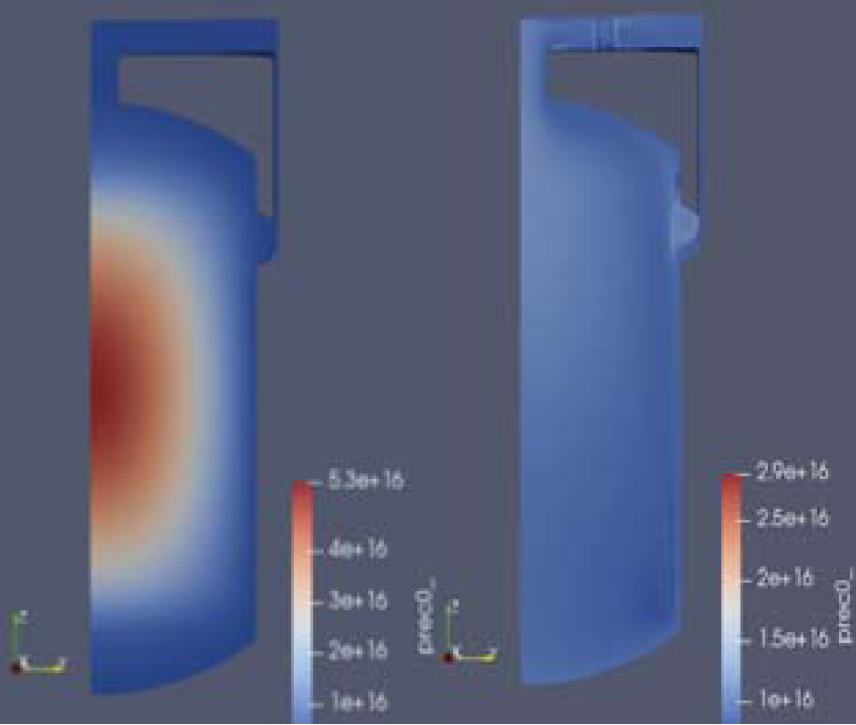
\includegraphics[scale=0.25]{images/dnp1.PNG}
  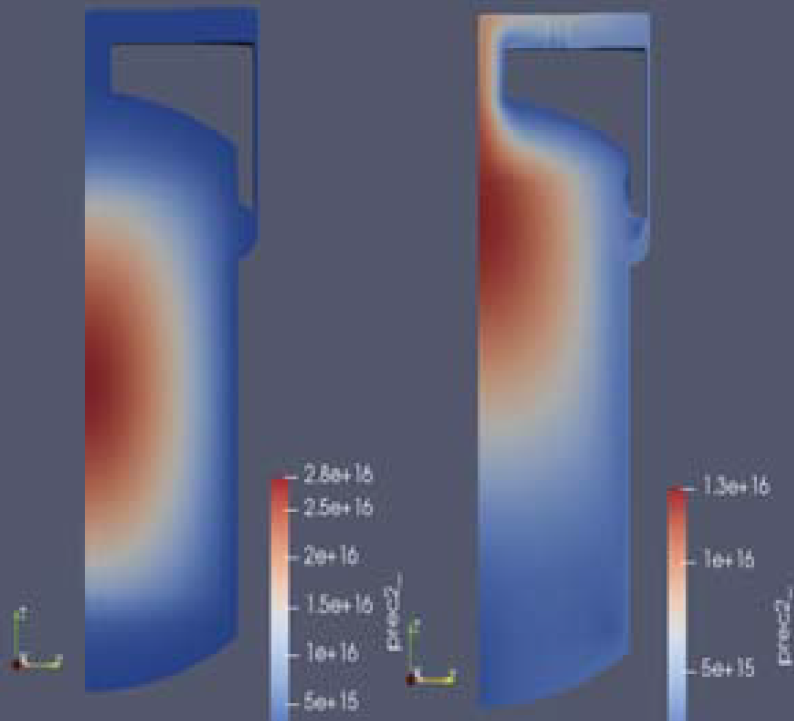
\includegraphics[scale=0.25]{images/dnp3.PNG}
  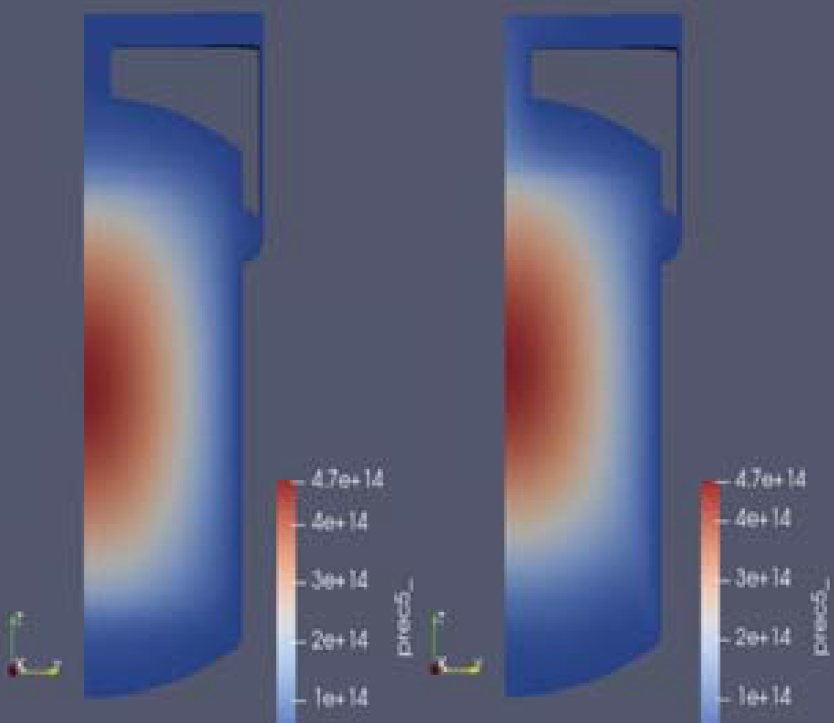
\includegraphics[scale=0.25]{images/dnp6.PNG}
  \caption{Plots of DNP concentrations in the molten salt reactor experiment \cite{shi_gen-foam_2021}. The left side of each image shows concentration with no flow, while the right shows the concentration with a 1200 gallon per minute flow rate. Top Left) Longest lived DNP group. Top Right) Third longest lived DNP group. Bottom) Shortest lived DNP group.}
   \label{fig:genfoam_dnp_locations}
\end{figure}

From these images, it can be seen that for the long shortest lived DNPs, the movement of the fuel does not have any significant impact upon the DNP distribution when compared to static fuel. This is reasonable since the precursors do not live for very long in this group, so they do not have much chance to travel. For the intermediate DNP group, there is a clear shift in the direction of the fuel flow, which causes more precursors to produce delayed neutrons in the less important piping  and upper plenum regions. The longest lived DNP group seems to be spread almost equally throughout the entire reactor, which means that those delayed neutrons are contributing significantly less to the overall neutron economy. This reduces the overall effective delayed neutron fraction since the delayed neutrons are in less important regions. This directly affects the controllability of the reactor through the reactor period, which is heavily dependent upon the delayed neutrons.

\section{Depletion}

Depletion is the process of burning the fuel and simulating the changes to the materials this causes in the system. Depletion requires specific information to run properly, such as decay constants,  fission yields, and fission and transmutation cross section data. The fission and transmutation cross section data can come from a transport calculation, while the other data can be read from a data library \cite{leppanen_development_2007}. Additionally, running depletion involves solving the Bateman equations, a generic version of which can be seen in Equation \ref{eq:Bateman_default}.

There are several different approaches to solving these equations, such as the Transmutation Trajectory Analysis (TTA) method and the Chebyshev Rational Approximation Method (CRAM). These are the two different methods used in Serpent2, and are both built into Serpent2 \cite{leppanen_serpent_2015}. Other codes may use external software to compute depletion, such as REM used by MCNP and ORIGEN-S used by KENO-VI \cite{aufiero_extended_2013}. Another code, aside from Serpent2, that contains built-in depletion solvers is ERANOS \cite{aufiero_extended_2013}.

The purpose behind solving these equations and having depletion models is to generate an accurate representation of the composition of the target materials during reactor operation. This is important in determining how long the reactor can run, how the safety of the reactor develops over time, and how operation may have to change to adjust to the new reactor state. For molten salt reactors, depletion also allows for information regarding fresh fuel feed rate and fission product removal rates, as well as how variations of those parameters can affect reactor performance and behaviour.

\section{The Molten Salt Breeder Reactor}

The molten salt breeder reactor (MSBR) is a useful design to analyze for several reasons. Because it is a molten salt reactor, online reprocessing is used within the design. In addition, it contains an inner and outer zone, each of which has different neutronic behaviour \cite{robertson_conceptual_1971}. More specifically, the inner zone has a softer spectrum, a higher fission rate, and a 13\% fuel-to-graphite ratio \cite{park_whole_2015}. The outer zone has a harder spectrum, a higher breeding rate, and a 37\% fuel-to-graphite ratio. The inner and outer zones prove to be an issue when accurately modeling using a unit-cell or one-region approach, as those models are unable to capture the different characteristics of each region \cite{rykhlevskii_modeling_2019}. The differences in the regions can also be seen in Figure \ref{fig:msbr_ryklev}, which allows for the difference in the fuel-to-graphite ratio to be visually noticeable.

\begin{figure}[H]
  \centering
  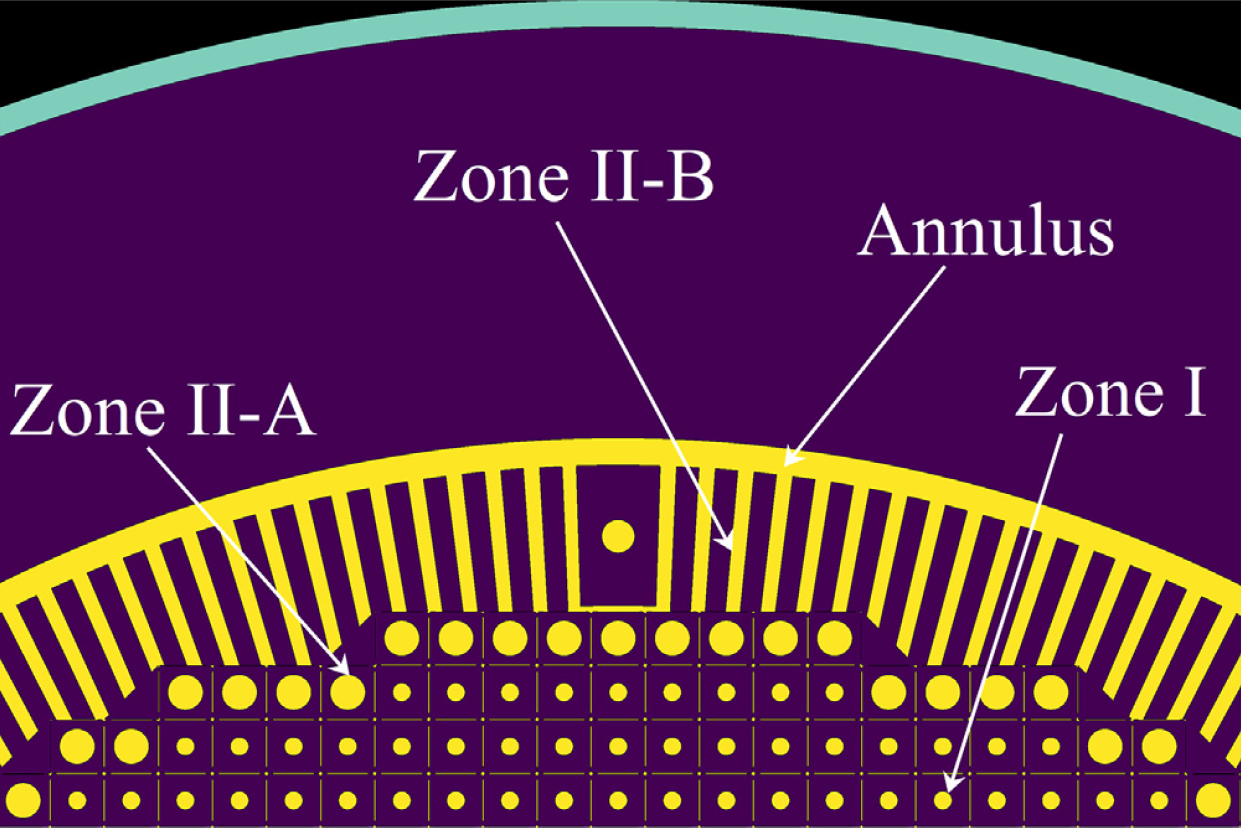
\includegraphics[scale=0.25]{images/msbr_ryk_1.PNG}
  \caption{MSBR core axial slice showing the different regions from \cite{rykhlevskii_modeling_2019}. Zones II-A and II-B are where the spectrum is harder and there is increased breeding. Zone I is where there is more fission and a softer spectrum. The yellow is fuel salt, the purple is graphite, and the cyan is the reactor vessel.}
   \label{fig:msbr_ryklev}
\end{figure}

Table \ref{tab:msbr_gen_data} has general information on the MSBR, while Table \ref{tab:msbr_salt_data} has specific information on the distribution of the fuel salt during operation. It can be seen in Table \ref{tab:msbr_gen_data} that the salt inventory cycle time is 10 days, which means that for the entire salt inventory to be cycled takes 10 days. However, the loop cycle time is 11 seconds \cite{robertson_conceptual_1971}.

\begin{table}[H]
\renewcommand{\arraystretch}{1.25}
\caption{MSBR General Data \cite{robertson_conceptual_1971}}
\label{tab:msbr_gen_data}
\begin{center}
\begin{tabular}{ | c | c | }
 \hline
 Component & Data\\
 \hline
 \hline
 Thermal Capacity & 2250 MW$_{th}$\\
 Vessel Inner Diameter & 6.77 m\\
 Core Height & 3.96 m\\
 Vessel Pressure & 0.52 MPa\\
 Inner Salt Fraction & 0.13\\
 Outer Salt Fraction & 0.37\\
 Maximum Flow Velocity & 2.6 $\frac{m}{s}$\\
 Fuel Salt (Vessel) & 30.4 m$^3$\\
 Fuel Salt (Primary System) & 48.7 m$^3$\\
 Thorium Inventory & 68,100 kg\\
 Breeding Ratio & 1.06\\
 Processing Rate & 1 gpm\\
 Salt Inventory Cycle Time & 10 days\\
 Salt Components & $\ce{^{7}LiF-BeF_{2}-ThF_{4}-UF_{4}} $\\
 Salt Composition & 71.7-16-12-0.3 mole \% \\
 \hline
\end{tabular}
\end{center}
\end{table}

Table \ref{tab:msbr_salt_data} shows that the salt inventory in the core is approximately 19 m$^3$ due to each core zone. However, SaltProc uses the volume of the primary system for its calculation \cite{rykhlevskii_modeling_2019}. This is because the other parts of the MSBR outside of the core are not modeled, but the geometry implemented in Serpent2 uses the correct dimensions. This allows cross sections to remain as if the correct volume were implemented, but also allows the depletion results to be closer to the expected result if the fuel salt were fully utilized.


\begin{table}[H]
\renewcommand{\arraystretch}{1.25}
\caption{MSBR Primary System Salt Inventory \cite{robertson_conceptual_1971}}
\label{tab:msbr_salt_data}
\begin{center}
\begin{tabular}{ | c | c | }
 \hline
 Region & Volume [m$^3$]\\
 \hline
 \hline
 Fuel Salt (Primary System) & 48.7\\
 \hline
 Reactor & -\\
 Core Zone I & 8.2\\
 Core Zone II & 10.8\\
 Plenums, Inlets, Outlets & 6.2\\
 Annulus & 3.8\\
 Reflectors & 1.4\\
 \hline
 Primary Heat Exchangers & -\\
 Tubes & 7.6\\
 Inlets, Outlets & 0.8\\
 \hline
 Pump Bowls & 5.2\\
 Piping (including drain line) & 4.1\\
 Off-gas bypass loop & 0.3\\
 Tank heels and miscellaneous & 0.3\\
 \hline
\end{tabular}
\end{center}
\end{table}


\begin{table}[H]
\renewcommand{\arraystretch}{1.25}
\caption{MSBR Online Reprocessing Cycle Times \cite{robertson_conceptual_1971}}
\label{tab:msbr_cycle_times}
\begin{center}
\begin{tabular}{ | p{0.27\linewidth} | p{0.25\linewidth} | p{0.35\linewidth} |}
 \hline
 Reprocessing Group & Element(s) & Cycle Time (Full Power)\\
 \hline
 \hline
 Rare Earths & Y, La, Ce, Pr, Nd, Pm, Sm, Gd & 50 days\\
 Rare Earths & Eu & 500 days\\
 Noble Metals  & Se, Nb, Mo, Tc, Ru, Rh, Pd, Ag, Sb, Te & 20 seconds\\
 Seminoble Metals & Zr, Cd, In, Sn &  200 days\\
 Gases & Kr, Xe & 20 seconds\\
 Volatile Fluorides & Br, I & 60 days\\
 Discard & Rb, Sr, Cs, Ba & 3435 days\\
 Salt Discard & Th, Li, Be, F & 3435 days\\
 Protactinium & Pa & 3 days\\
 Higher Nuclides & Np, Pu & 16 years\\
 \hline
\end{tabular}
\end{center}
\end{table}


%Pa233, Np237, Pu242

Shown in Table \ref{tab:msbr_cycle_times} are the cycle times for different elements in the MSBR. According to Robertson et al, the protactinium and rare earth processing has the largest impact on neutronics and performance \cite{robertson_conceptual_1971}. 

The fuel processing of the MSBR is defined to operate continuously with processing methods \cite{robertson_conceptual_1971}. For protactinium removal, fluorination is first used to remove uranium before protactinium isolation. Next is countercurrent bismuth with lithium and thorium for stripping any remaining uranium and the protactinium. This is followed by hydrofluorination to separate the uranium and protactinium. This process can be seen in Figure \ref{fig:msbr_pa}. For a 10 day protactinium cycle time, a fuel salt flow rate of 0.88 gallons per minute (gpm) is used. The processed salt is processed for rare earth fission products before being fed back into the reactor. 
% Page 111 flow sheet
\begin{figure}[H]
  \centering
  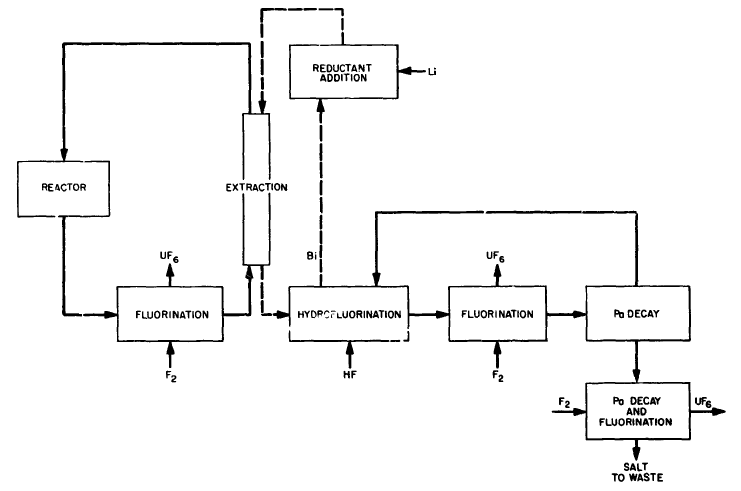
\includegraphics[scale=0.55]{images/msbr_pa_robertson.PNG}
  \caption{MSBR protactinium processing scheme from Robertson et al \cite{robertson_conceptual_1971}.}
   \label{fig:msbr_pa}
\end{figure}

Rare earth fission product removal is performed using the metal-transfer process, which uses lithium chloride and bismuth containing a reductant. More specifically, bismuth containing a reductant of thorium and lithium is used to strip the rare earth fission products from the fuel salt. The rare earth fission products are then transported to the lithium chloride acceptor salt, though lithium bromide or a mix of both could be used. Figure \ref{fig:msbr_re} shows this process, and Figure \ref{fig:msbr_re_pa} shows the protactinium and rare earth processing schemes together.

\begin{figure}[H]
  \centering
  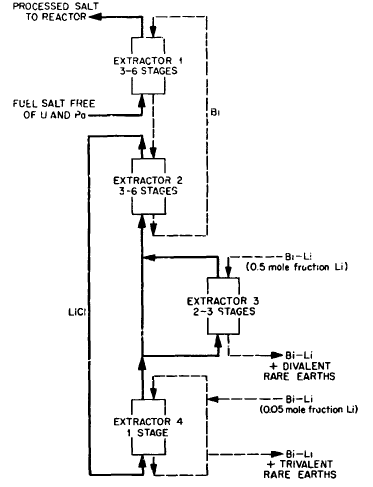
\includegraphics[scale=0.65]{images/msbr_re_robertson.PNG}
  \caption{MSBR rare earth processing scheme from Robertson et al \cite{robertson_conceptual_1971}.}
   \label{fig:msbr_re}
\end{figure}

\begin{figure}[H]
  \centering
  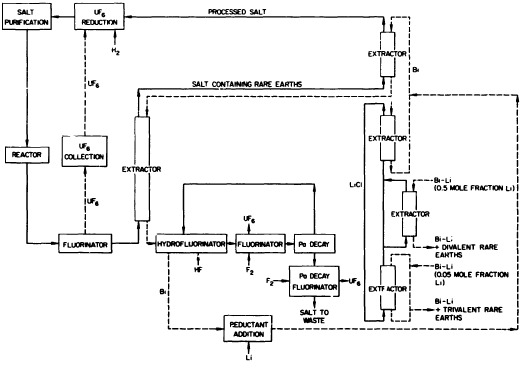
\includegraphics[scale=0.75]{images/msbr_flows_robertson.PNG}
  \caption{Combined MSBR rare earth and protactinium processing schemes from Robertson et al \cite{robertson_conceptual_1971}.}
   \label{fig:msbr_re_pa}
\end{figure}

To strip gaseous fission products, a bubble generator introduces sparging gas in 15 to 20 mil bubbles. 10 percent of the flow is redirected to the bypass loop which contains a gas separator. This gas separator strips the fission products with approximately 100 percent efficiency. The off-gas system also includes an approximately 2 hour holdup during which noble metals deposit on the fuelsalt drain tank surface. Figure \ref{fig:msbr_nm_pa} shows this process, beginning with the number per time, or flux, of the noble gasses in the salt migrating to the graphite voids and helium sparging bubbles. This is followed by the volume holdup into more processing to handle the noble metal fission product cleanup.

\begin{figure}[H]
  \centering
  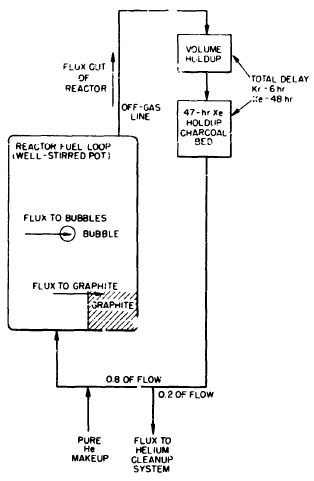
\includegraphics[scale=0.65]{images/msbr_nm_robertson.PNG}
  \caption{MSBR noble metal flux and off-gas system from Robertson et al \cite{robertson_conceptual_1971}.}
   \label{fig:msbr_nm_pa}
\end{figure}

Periodic discard of salt at a rate of 0.1 cubic feet per day occurs due to buildup of non-volatile fluorides during fluorination accumulating in the decay tank, such as from zirconium and corrosion product nickel.

%From SaltProc's MSBR example, the removal of each group can be attributed to a particular process within the physical system \cite{rykhlevskii_modeling_2019}. The entrainment separator is used to remove the gases; a nickel mesh is used to remove noble metals, seminoble metals, and volatile fluorides; and various processes given by Robertson are lumped together into the liquid metal process which removes rare earths, discard, and protactinium \cite{robertson_conceptual_1971}. The higher nuclides are removed at such an infrequent rate that they are not included within the SaltProc processes. The MSBR design removes the protactinium with the intent that the protactinium-233 will not absorb neutrons and will instead be fed out of the core to decay into uranium-233, which can then be fed back into the core.


\section{MSR Modeling Approaches}

For modeling of MSRs, there are generally two different models which are used. The first is a model which takes a given fuel composition and analyzes the performance of the reactor given that fuel composition. This may include focus on aspects such as DNP movement \cite{fei_molten_2020, shi_gen-foam_2021} or reactor dynamics \cite{singh_plant-level_2020, cervi_development_2019, aufiero_development_2014, cui_development_2022, singh_dynamics_2017}.

The second type of model is one which depletes the fuel. Because the online reprocessing of an MSR has such large effects on its fuel composition, depletion models of MSRs typically incorporate online reprocessing. These models can also account for other factors, such as DNP movement, as shown by Zhou et al \cite{zhou_fuel_2018}. The movement of DNP can have a noticeable effect on reactor performance by affecting neutron energy spectra and distribution of delayed neutrons \cite{betzler_implementation_2017}. Most, however, focus primarily on depletion and do not consider the DNP movement during depletion, as can be seen in Table \ref{tab:codes_types}. In order to handle spatial dependence of fuel salt without modeling the piping of the core, models can use the scaled flux method \cite{betzler_liquid-fueled_2021}.

For all of the continuous reprocessing models given in Table \ref{tab:codes_types}, all of them use the "fictitious decay constant" approach, which is shown in Equation \eqref{eq:Bateman_type_one_decay}. For the batchwise models, they typically use the approach shown in Equation \eqref{eq:batchwise_rem_eff} and remove a fraction at each depletion step rather than bulk removal at certain steps.

The "Reprocessing" column of Table \ref{tab:codes_types} shows the mathematical approach taken to the online reprocessing of the work, and does not necessarily represent the reactor reprocessing approach. However, since online reprocessing is considered in the table, offline batchwise reprocessing is not included, such as in the work by Zou et al \cite{zou_transition_2020}.

%For modeling of MSRs, there are typically three main types of models which are used. The first is a model which takes a fuel composition and runs without accounting for reprocessing, but accounts for the fuel movement effects, such as DNP drift, shown by Fei et al \cite{fei_molten_2020}. The second is a model which accounts for both fuel movement and reprocessing, such as Zhou et al \cite{zhou_fuel_2018}. The third is a model which does not account for fuel movement but accounts for reprocessing. Models which use the second or third approach are detailed in Table \ref{tab:codes_types}.


% Remove scale and step columns from table, include in description of model
\begin{table}[H]
\renewcommand{\arraystretch}{1.25}
\caption{Molten Salt Reactor Models with Online Reprocessing}
\label{tab:codes_types}
\begin{center}
\begin{tabular}{ | c | c | c | c | c | c | c | c | }
 \hline
 Index & Reprocessing & Model & Reactor & DNP & Ref.\\
 \hline
 \hline
 1 & Batchwise & Full 3D & MSBR & No & \cite{rykhlevskii_modeling_2019}\\
 2 & Continuous & Full 3D & MSFR & No & \cite{aufiero_extended_2013}\\
 3 & Batchwise & Full 3D & MSBR & No & \cite{park_whole_2015}\\
 4 & Batchwise & Unit Cell & MSBR & No & \cite{betzler_molten_2017}\\
 \;\,4* & Continuous & Unit Cell & N/A & No & \cite{jr_vicente_valdez_modeling_2020}\\
 5 & Batchwise & Unit Cell & DMSR & No &  \cite{ahmad_neutronics_2015}\\
 6 & Continuous & Full 3D & MSBR & Yes & \cite{zhou_fuel_2018}\\
 7 & Batchwise & Full 3D & MSBR & No & \cite{nuttin_potential_2005}\\
 8 & Batchwise & Full 3D & MOSART & No & \cite{sheu_depletion_2013}\\
 9 & Continuous & Unit Cell & ADNA & No & \cite{rodriguez-vieitez_transmutation_2002}\\
 10 & Mixed & 2D Slice & MSFR & No & \cite{fiorina_preliminary_2012}\\
 11 & Continuous & Full 3D & MSFR & No & \cite{zhuang_extended_2020}\\
 12 & Batchwise & Full 3D & Toy & No & \cite{ridley_method_2017}\\
 13 & Mixed & 2D Slice & N/A & Yes & \cite{h_f_bauman_rod_1971}\\
 14 & Mixed & Full 3D & TMSR & No & \cite{merle-lucotte_thorium_2007}\\
 15 & Mixed & Unit Cell & Toy & Yes & \cite{nagy_parametric_2008}\\
 16 & Continuous & Full 3D & N/A & No & \cite{xia_development_2019}\\
 \hline
\end{tabular}
\end{center}
\end{table}

The first entry in Table \ref{tab:codes_types} is SaltProc's MSBR example, which uses Serpent2, a full 3D core, 3 day time steps, and runs for 60 years. The batchwise reprocessing in SaltProc includes both the removal and feed processes.

The second entry is by Aufiero et al, and displays the Serpent2 newly developed continuous reprocessing functionality. A full 3D simplified core layout of the molten salt fast reactor (MSFR) is used, and continuous reprocessing is used to operate the removal and feed processes. It evaluates the model at various scales, from steady state uranium concentrations at over 60 years to radiotoxicity over $10^8$ years. The step sizes vary as well, though not specifically mentioned, appearing very small at BOC and expanding to around 10 years at SS for one of the figures presented.

The third entry by Park et al is very similar to the MSBR example in SaltProc, with the primary difference being MCNP6 is used for transportation calculations instead of Serpent2. The depletion was performed using CINDER90 and custom Python scripts. Another difference is that SaltProc uses adjusted values for the removal efficiency rates of xenon, krypton, and protactinium, while the work by Park et al uses the cycle time values from Robertson et al \cite{robertson_conceptual_1971}. This model uses 3 day time steps and models the fuel composition over 20 years.

The fourth entry is for ChemTriton, a tool designed for SCALE to perform online reprocessing of MSRs. It contains work on multiple reactors, such as the MSBR and the MSRE. The tool iteratively runs SCALE/TRITON over small time steps to simulate continuous reprocessing. For the MSBR case, 3 day time steps are used, similar to SaltProc and Park et al. The reason for not using shorter time steps is that using shorter time steps increases computational cost while also providing very little improvements to calculated eigenvalue and fuel cycle metrics, discussed by Betzler et al as well as by Powers et al \cite{powers_new_2013}.

ChemTriton has been updated after TRITON implemented new tools for continuous material feeds and removals. The work discusses in depth how the removal rates for isotopes can be calculated using a well mixed approximation and accounting for non-modeled piping by introducing a correcting decay factor. Although it does not account for DNP movement, it does account for neutron important regions without having to model the piping regions.

The fifth entry by Ahmad et al analyzes single fluid and two fluid denatured molten salt reactors (DMSRs). This work uses MCNP5 and ORIGEN2 as the codes to perform transport and depletion over 30 years. Although the steps at which fuel is adjusted is at 5 year intervals, the burnup intervals are actually set to 6 months. The reason such large steps were used is because the work analyzes proliferation and resource requirements for the reactors. This means that the neutronics and safety parameters were not as important, and so the model did not have to be as precise in that regard. Additionally, only gaseous fission products or fission products which are removed via sparging are included in the reprocessing scheme, no other chemical extraction takes place. This is because the authors wanted the system to be as simple as possible. ORIGEN provides continuous reprocessing capability, however for this work it would not have been necessary since the authors wanted to use a simpler approach for the model \cite{gauld_isotopic_2011}.

The sixth entry by Zhou et al is for FAMOS (Fuel cycle Analysis code for MOlten Salt reactors). This code uses OpenMC to generate homogenized cross section data followed by the DIF3D diffusion solver along with extensions to model DNP movement, thermal hydraulics, depletion, and continuous reprocessing. Their work also analyzes the molten salt fast reactor over 200 operational years. The depletion step size is not specifically given in the work, but from analysis of the plots, small time steps seem to have been used at the beginning of cycle and then larger time steps of ~100 days are then used for the rest of the steps.

The seventh entry by Nuttin et al analyzes the MSBR using a slightly simplified geometry with MCNP. The reprocessing approach used here is also the same as the approach used in SaltProc, which is to take the inverse of the cycle time to determine the removal rate. Depletion is performed in this work by coupling MCNP to an evolution program and the NJOY code. However, this work uses 10 day steps instead of 3 day steps that SaltProc uses. It also runs for 100 years instead of 20.

The eight entry by Sheu et al analyzes the Molten Salt Actinide Recycler \& Transmuter (MOSART) reactor and uses custom scripts to implement batchwise reprocessing. The codes used are SCALE6 for transport and TRITON for depletion. The step sizes used include 15, 30, and 60 days, in which the authors found that 30 days gave the best results in terms of accuracy and run time balancing for the 30 year simulation.

The ninth entry by Rodriguez-Vieitez analyzes the Accelerator-Driven Neutron Applications (ADNA) Tier-1 reactor using MCNP. Although the model used does implement continuous reprocessing in the Bateman equation, it is not used for the purpose of fuel cycle analysis and depletion. Rather, the work iteratively works towards the equilibrium fuel composition in order to analyze the effect of varying different reactor parameters, such as geometry.

The tenth entry by Fiorina et al is on the Molten Salt Fast Reactor (MSFR) and uses a modified version of the ERANOS-based EQL3D procedure. This model makes use of continuous reprocessing for non-soluble fission products, but uses batchwise reprocessing for soluble fission products. The batchwise reprocessing was incorporated for simplicity in the model. The time steps used are shorter at beginning of cycle at extend out to ~30 year steps for a 200 year depletion. Additionally, the radiotoxicity analysis extends out to 1 million years.

The eleventh entry by Zhuang et al discusses an OpenMC extension called OpenMCB-MSR to implement continuous reprocessing in an analysis of the MSFR. The depletion step sizes used are not specified in the work, though with continuous reprocessing step sizes could have been set to above single digit days and still maintained high precision.

The twelfth entry by Ridley and Chvala use batchwise reprocessing on a toy MSR using Serpent2 and a python library. The feed rates were set to fluctuate in order to maintain criticality while also accounting for density imbalance in Serpent2 by increasing the volume of the material. The full core 3D model was then analyzed using 7 day depletion steps for 10 years.

The thirteenth entry is on the Reactor Optimum Design (ROD) code, which allows users to use continuous or batchwise reprocessing for the MSR model. ROD operates by taking a one or two dimensional input and determining the equilibrium fuel composition. This is a useful code for determining a prediction of a model, but is less precise than more modern codes which offer more detailed geometry and other features.

The fourteenth entry by Merle-Lucotte et al covers depletion of the Thorium Molten Salt Reactor (TMSR) using MCNP4 \cite{goluoglu_software_1998} for transport and REM for material evolution. Continuous reprocessing is used for gaseous fission product extraction, while the other fission products are processed with batchwise reprocessing.

The fifteenth entry by Nagy et al uses a toy model to go through different reprocessing schemes based on the MSBR and MOSART reprocessing designs \cite{robertson_conceptual_1971, ignatiev_progress_2007}. SCALE-5 \cite{noauthor_scale_2005} is used for neutron transport and ORIGEN-S is used for depletion. To account for DNPs, the authors make a few approximation which lead to reducing the calculated eigenvalues by 90 pcm. Depeletion steps are performed every 5 days, during which continuous reprocessing was implemented for either only gaseous fission product removal or more, depending on the reprocessing scheme chosen. Additionally, the batchwise reprocessing was performed by altering the binary output of ORIGEN, as is performed for the feed fuel and more, depending on the reprocessing scheme chosen.

The sixteenth entry by Xia et al demonstrates the MOlten salt reactor specific DEpletion Code (MODEC). This code uses continuous reprocessing, and has been used to analyze the Molten Chloride salt Fast Reactor (MCFR) by Liaoyuan et al \cite{liaoyuan_th-u_2021}. The MCFR analysis uses SCALE6.1 for transport and MODEC for depletion. 


\chapter{Methods}
\renewcommand*\descriptionlabel[1]{\hspace\leftmargin$#1$}
\setcounter{tocdepth}{5}
\setcounter{secnumdepth}{5}

%\section{Notes}

%A 1-gpm
%(0.06 liter/sec) side stream of the primary salt is
%continuously processed to remove
% 233 P a , to recover the
%bred
% 233 U , and to adjust the fissile content. Robertson summary

% Robertson does not define thorium feed rate?

% Serpent2 continuous reprocessing section cite own presentations at Serpent user group meetings

In this chapter, I will discuss the methodology used for the different reprocessing schemes, mass balancing, delayed neutron precursors, and the Serpent2 model used in this work.
More specifically, I will describe in detail first two different approaches for batchwise reprocessing which have been implemented in SaltProc, the tool used in this work to handle batchwise reprocessing \cite{rykhlevskii_saltproc_2018}. I will then give a summary of the two approaches and provide estimates for the expected error and computational costs compared to continuous methods.

After that, I will then discuss three different continuous reprocessing methods, while focusing heavily on one.
Within this particular method, I will discuss several approaches which can be implemented.

Finally, I will provide information on the mass balancing, effects of delayed neutrons on depletion results, and the Serpent2 model used to generate results.

\section{Batchwise Reprocessing}
\label{s:batch-generic}

As previously mentioned in Section \ref{s:SP-repr}, SaltProc has two different versions which use two different batchwise reprocessing approaches.
These approaches are the Bulk batchwise approach, used in version 0.1 of SaltProc, and the Steady batchwise approach, used in version 0.3 of SaltProc.
%SaltProc is used to handle batchwise reprocessing in this work because it provides a batchwise reprocessing scheme which can be customized fairly easily.
%SaltProc is used to handle batchwise reprocessing in this work because it uses Serpent2, which has built-in continuous reprocessing; comes with the MSBR geometry in Serpent2 as an example; and has multiple versions.
%Of these different versions of SaltProc, they have slightly different methods in how the depletion data is stored as well as how reprocessing rates are calculated.
%However, the two versions of interest are version 0.1 and 0.3, which use different batchwise reprocessing approaches.
%These two different approaches are referred to here as the "Bulk" approach and the "Steady" approach.
%which
%an accurate model of the MSBR, uses Serpent2 for transport and depletion calculations, and because it provides

\subsection{Bulk}

%SaltProc version 0.1 was the first full version of SaltProc publicly released, and provides all the functionality necessary for modeling the MSBR with batchwise reprocessing.
%Using this version, Rykhlevskii uses three day depletion steps and does not perform fractional reprocessing at each step, instead performing reprocessing according to the cycle times \cite{rykhlevskii_advanced_2018}.
%This approach is termed as the "Bulk" approach to batchwise reprocessing, and is explained in more detail below. This is the same approach used by Gehin and Powers for an analysis of the MSBR \cite{gehin_liquid_2016}.

The Bulk approach operates by not performing any reprocessing until the cycle time, or time it takes for a given element to be completely removed, is met or exceeded.
At that point, 100\% of the target is removed.
For example, imagine a simulation with a three day depletion step size. An element with a 30 day cycle time would have no reprocessing during the first 27 days, then full 100\% removal of the target at the 30 day mark. This works well for reactor processes which are performed batchwise, such as adding uranium to the reactor which can be performed as a batch process. However, for approximating online reprocessing, this approach is not ideal, as it is less able to capture the frequency of the reprocessing.

For the refueling of the reactor, the thorium feed rate was set to maintain the thorium mass in the reactor. The uranium feed rate was set to be equivalent to the protactinium removal rate. This carries an implicit assumption that there is already a backlog of decayed protactinium which has transmuted into uranium which is ready to be pumped back into the core. Both the thorium feed and protactinium to uranium refueling processes occur every 3 days. These refueling rates can be seen in Figures \ref{fig:Th-feed-v1} and \ref{fig:U-feed-v1}, which are recreated from the data from Rykhlevskii \cite{rykhlevskii_advanced_2018}.

% Include figure of U and Th feed rates over time.

\begin{figure}[H]
  \centering
  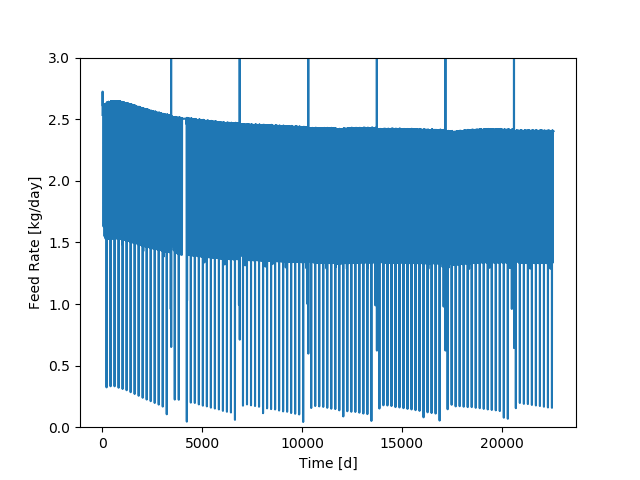
\includegraphics[scale=0.75]{images/Th232rem_massv01.png}
  \caption{Thorium feed rate in the MSBR as a function of time while using Bulk batchwise reprocessing \cite{rykhlevskii_advanced_2018}.}
   \label{fig:Th-feed-v1}
\end{figure}

\begin{figure}[H]
  \centering
  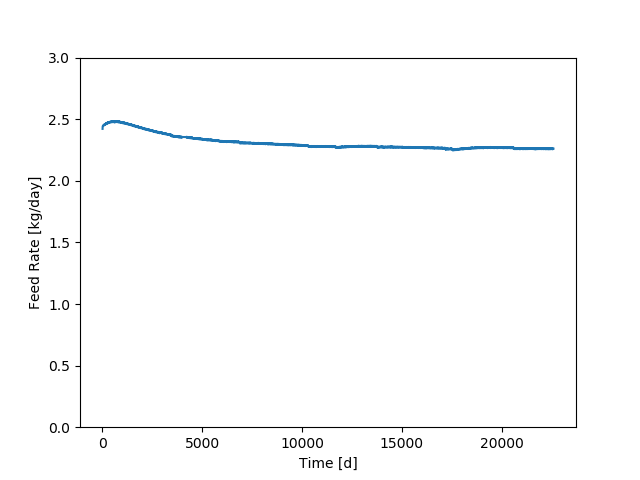
\includegraphics[scale=0.75]{images/Pa233rem_massv01.png}
  \caption{Uranium feed rate in the MSBR as a function of time while using Bulk batchwise reprocessing \cite{rykhlevskii_advanced_2018}.}
   \label{fig:U-feed-v1}
\end{figure}

The large jumps in the thorium feed rate are due to the bulk removal of rubidium, strontium, caesium, and barium; this causes jumps in the thorium feed rate because the thorium feed rate in this version of SaltProc is based on mass balancing.
Removing a large amount of fission products results in that mass being replaced by thorium.
This also leads to spikes in the effective multiplication factor, as the removal of the fission products inserts more reactivity than the addition of thorium removes \cite{rykhlevskii_advanced_2018}. The uranium feed rate is smooth because it is based purely on the outflow of protactinium and does not fluctuate as rapidly as the thorium, which is the only external feed in the MSBR system. The average thorium-232 feed rate is 2.38 kg/day, while the average uranium-233 feed rate is 2.31 kg/day. These average values are used as the baseline for the feed rates in the rest of this work.

\subsection{Steady}
\label{s:steady}

%SaltProc version 0.3 includes an example MSBR which users can run as soon as SaltProc is installed, though some of the run parameters such as neutrons per generation and run time have to be altered to generate a more valid model. This model also uses 3 day steps, but instead of performing the batch removal only at the cycle time value, this model removes a fraction every 3 days, which is called the "Steady" approach for batchwise reprocessing.
Steady batchwise removes a fraction of the target at each depletion time step rather than 100\% removal at certain time steps.
For example, a 30 day cycle time would result in 10\% removal every 3 days. This more accurately models online reprocessing, which is primarily what the MSBR employs in its reprocessing scheme. However, this steady version of SaltProc also makes some minor changes to the reprocessing scheme by adding in efficiency terms. These changes act as a multiplier on the reprocessing constant, where 100\% efficiency makes no change and 0\% makes the reprocessing constant become 0. These changes are as follows: xenon uses 91.2\% removal over three days instead of 100\%, krypton uses 91.5\% removal over three days instead of 100\%, protactinium uses 9.5\% removal over three days instead of 100\%, and the discard has a removal of 0.9\% over three days instead of 0.09\%.

The reactor refueling is performed slightly differently from v0.1 as well. This version assumes a constant ratio between the uranium refueling and the thorium refueling. The net refueling for each 3 day depletion step is set to maintain the mass of the system. Thus, the average values of 2.38 kg/day and 2.31 kg/day for thorium-232 and uranium-233, respectively, are used to determine the ratio of uranium to thorium which is implemented.

Figures \ref{fig:Th-feed-v3} and \ref{fig:U-feed-v3} show the refueling rate of thorium-232 and uranium-233, respectively, using a depletion step size of 3 days over a net time of 90 days. The average feed rates of the thorium-232 and uranium-233 are 1.24 and 1.21 kg/day. The reasons for the difference are because the smaller efficiencies cause less mass loss, a shorter time frame is covered, and the protactinium removal is much less, resulting in a much smaller uranium-233 feed.

\begin{figure}[H]
  \centering
  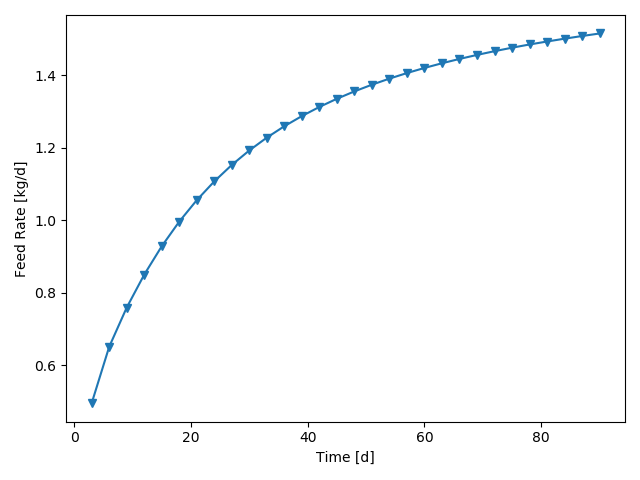
\includegraphics[scale=0.75]{images/feed_Th232_3d_90d.png}
  \caption{Thorium feed rate with a depletion time step of 3 days in the MSBR as a function of time while using Steady batchwise reprocessing.}
   \label{fig:Th-feed-v3}
\end{figure}

\begin{figure}[H]
  \centering
  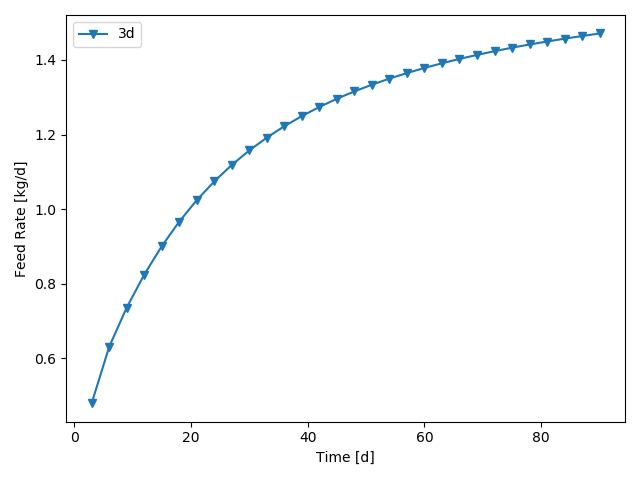
\includegraphics[scale=0.75]{images/feed_U233_3d_90d.png}
  \caption{Uranium feed rate with a depletion time step of 3 days in the MSBR as a function of time while using Steady batchwise reprocessing.}
   \label{fig:U-feed-v3}
\end{figure}

%Additionally, this version of SaltProc uses the PyTables Python package for handling the hdf5 data files. The data files are structured similarly to v0.1 of SaltProc, but instead of atom density they use mass, which makes analysis of the files slightly more user friendly.

\subsection{Batch Approaches Summary}
\label{s:batch-sum}

\begin{table}[H]
\renewcommand{\arraystretch}{1.25}
\caption{Batchwise Reprocessing Methods}
\label{tab:batch_methods}
\begin{center}
\begin{tabular}{ c | c | c | c | c }
 \hline
        Approach & $\Delta t$ $[s]$ & $T_{cyc}$ $[s]$ & Fractional Removal Rate [s$^{-1}$] & Step Removal\\
 \hline
 \hline
        Bulk & 1 & 20 & - & \, 0/1$^{*}$\\
        Bulk & 10 & 20 & - & \, 0/1$^{*}$ \\
        Bulk & 40 & 20 & - & 1 \\
        Steady & 1 & 20 & 0.05 & 0.05\\
        Steady & 10 & 20 & 0.05 & 0.5\\
        Steady & 40 & 20 & 0.025 & 1\\
 \hline
\end{tabular}
\end{center}
\end{table}
        \begin{center}
\footnotesize{$^{*}$ Bulk removal is 0 until the depletion step is equal to the cycle time, at which point it removes 100\%.}\\
        \end{center}

Table \ref{tab:batch_methods} reflects the information shown in Figure \ref{fig:bulk_repr_cnst}. The table shows how the Bulk method will only remove 100\% at the cycle time, and otherwise removes nothing. Additionally, the Bulk method will remove 100\% as soon as possible if the depletion step size, $\Delta t$, is larger than the cycle time, $T_{cyc}$.

The table also describes how the Steady method fractional removal is constant up until the depletion step size becomes larger than the cycle time, at which point the removal at each step is 100\%, causing the Steady method to then be equivalent to the Bulk method. However, for shorter times, the Steady method allows for a consistent fractional removal rate by adjusting the removal at each step.


\begin{figure}[H]
  \centering
  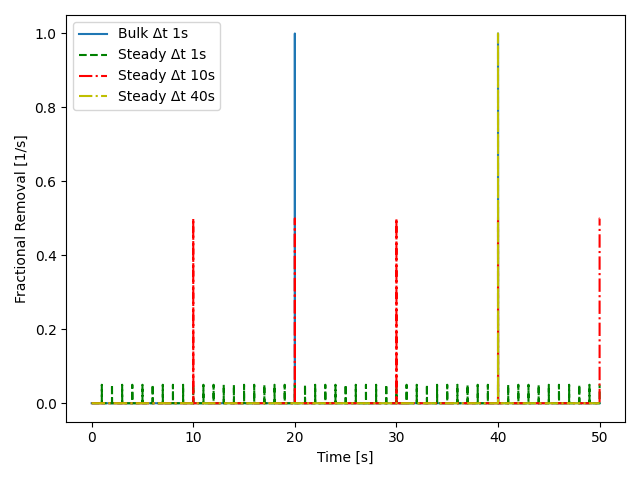
\includegraphics[scale=0.75]{images/bulk-compare-cycles.png}
  \caption{Plot showing how Bulk and Steady batchwise reprocessing removal works as a function of time for an example with a cycle time of 20 seconds.}
   \label{fig:bulk_repr_cnst}
\end{figure}

Figure \ref{fig:bulk_repr_cnst} shows an example fractional removal scheme for a fission product with a cycle time of 20 seconds. The Bulk method simply extracts 100\% of the product every 20 seconds, no matter how small the depletion step size is. The Steady method removes some fraction every depletion step, which allows a semi-continuous process as the depletion step size becomes smaller and smaller. This can be seen in how a 10 second depletion step results in 50\% removal every 10 seconds, whereas a 1 second step allows for 5\% removal per depletion step.


% Add comparison of batch/steady for matrix of possible combinations.

\begin{figure}[H]
  \centering
  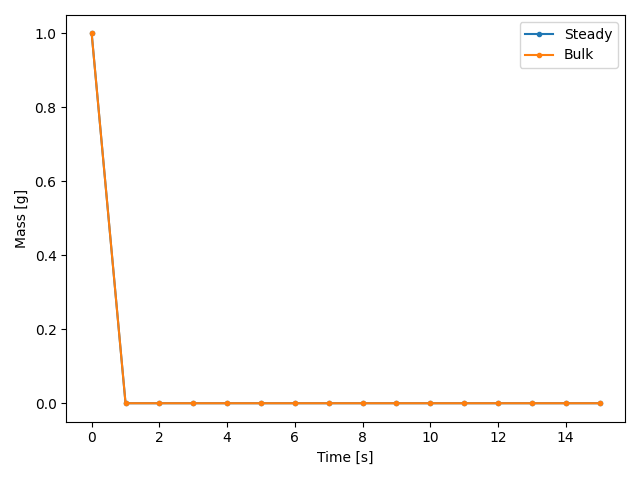
\includegraphics[scale=0.75]{images/batch-steady-identical-compare.png}
  \caption{Plot showing how Bulk and Steady batchwise reprocessing are identical while the cycle time is shorter than or equal to the depletion step size.}
   \label{fig:bulk_repr_comp}
\end{figure}

A useful piece of information to note is that if the cycle time is shorter than or equal to the depletion step size, then the Steady and Bulk batchwise methods will be identical to each other, as demonstrated in Figure \ref{fig:bulk_repr_comp} which shows a simple model case with 1 second depletion steps and 1 second cycle times for an imaginary isotope. For the MSBR simulation, this means that the noble metals, gasses, and protactinium reprocessing will remain the same for either batchwise method employed. However, the longer cycle time groups such as the rare earths and volatile fluorides have cycle times which are 10-20 times longer than the depletion step size.

Figure \ref{fig:bulk_repr_diff} shows a simulation of this for a situation where an isotope is generated at a rate of 1 gram per second, and is simulated with some combination of cycle time and depletion step size where the depletion step size is smaller than the cycle time.

\begin{figure}[H]
  \centering
  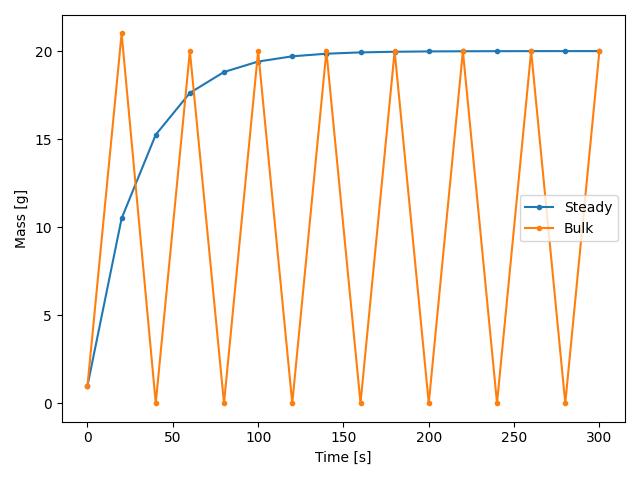
\includegraphics[scale=0.75]{images/batch-40-20.png}
  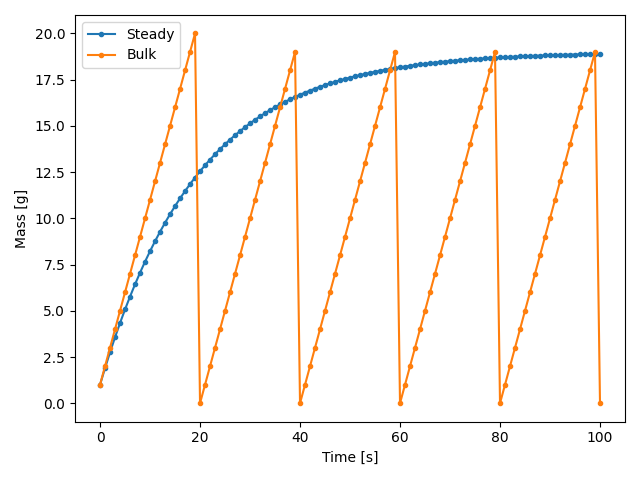
\includegraphics[scale=0.75]{images/batch-20-1.png}
  \caption{Plot showing how Bulk and Steady batchwise reprocessing are different while the cycle time is longer than the depletion step size for a 40 second cycle time and 20 second depletion step (top) and a 20 second cycle time with a 1 second depletion step (bottom).}
   \label{fig:bulk_repr_diff}
\end{figure}

One interesting aspect to note from this figure is that the Steady method approaches a steady state value which is at the peak of the Bulk method. This result can be confirmed by checking that the solutions for both the Steady and Bulk methods are valid. To check the solution, the 40 second cycle time and 20 second depletion step will be used.

For the Bulk method, after 100\% removal after the first cycle time, or 40 seconds, the mass then oscillates between 20 and 0 grams. This makes sense since 20 grams are generated over 20 seconds while every 40 seconds there is 100\% removal.

For the Steady method, the initial mass of 1 gram gains 20 grams over 20 seconds, yielding 21 grams. However, the Steady removal then requires removal of 50\%, previously discussed and shown in Figure \ref{fig:bulk_repr_cnst}. This 50\% removal then drops the mass to 10.5 grams. 20 more grams are added to this value and 50\% is removed again, continuing iteratively. This can then be re-written as an infinite sum in order to determine the steady state solution. The first three iterations are shown in Equations \eqref{eq:ss-mass-p1} and \eqref{eq:ss-mass-p2}, where the value of 20 is the mass added during each depletion step and the value of 0.5 is the fractional removal performed each depletion step.
%In the generic form, the $C$ term represents the gain per second, $\Delta t$ is the depletion step size, and $T_{cyc}$ is the cycle time.

%\begin{equation} \hfill
%m_{n+1} = (m_n + C \Delta t) (1 - \frac{\Delta t}{T_{cyc}})
%\hfill\label{eq:ss-mass-p5-steady-generic} \end{equation}

\begin{equation} \hfill
m_{ss} = (((N_0+20)(0.5)+20)(0.5)+20)(0.5) + ...
\hfill\label{eq:ss-mass-p1} \end{equation}

\begin{equation} \hfill
m_{ss} = 0.5^3 N_0 + 0.5^3 (20) + 0.5^2 (20) + 0.5 (20) + ...
\hfill\label{eq:ss-mass-p2} \end{equation}

Continuing this form infinitely yields Equation \eqref{eq:ss-mass-p3}, where the infinite sum yields 1, resulting in a net value of 20, the result of which is unaffected by the initial mass of the isotope and instead depends on the generation and reprocessing rates.

\begin{equation} \hfill
m_{ss} = 20 \sum_{n=1}^\infty \frac{1}{2}^n
\hfill\label{eq:ss-mass-p3} \end{equation}

In order to generate a generic form for this equation, a short derivation is required, which is provided in Appendix A. From this derivation, Equation \eqref{eq:nplusone-gen} is generated.

\begin{equation} \hfill
m_{n+1} = \left[ \left(m_n + \frac{C}{\lambda - \lambda_r} \right)e^{-(\lambda - \lambda_r) \Delta t} + \frac{C}{\lambda - \lambda_r} \right] \left(1 - \Delta t \lambda_r \right),
\hfill\label{eq:nplusone-gen} \end{equation}

% Add generic form (x added per second, y removal rate)A more generic form for the case of a constant rate of change over each depletion step can be seen in Equation \eqref{eq:ss-mass-p4}.
In this equation, $C$ represents the gain terms in the Bateman equation, $\Delta t$ represents the depletion step size, $\lambda$ represents the loss terms in the Bateman equation, $\lambda_r$ represents the reprocessing constant. This equation assumes a constant $C$, $\lambda$, and $\lambda_r$, which is a reasonable assumption at steady state when the changes over time are negligible. This equation is used to generated the steady state equation as shown in Equations \eqref{eq:ss-mass-p4prev} through \eqref{eq:ss-mass-p4}.

%\begin{equation} \hfill
%m_{ss} = C \Delta t \sum_{n=1}^\infty \left( 1 - \frac{\Delta t}{T_{cyc}} \right)^n
%\hfill\label{eq:ss-mass-p4prev} \end{equation}

\begin{equation} \hfill
m_{ss} =  \frac{C}{\lambda - \lambda_r} \left(e^{(\lambda - \lambda_r) \Delta t} - 1 \right) \sum_{n=1}^{\infty} \left( \left(1 - \lambda_r \Delta t \right) e^{-(\lambda - \lambda_r) \Delta t} \right)^n
\hfill\label{eq:ss-mass-p4prev} \end{equation}

\begin{equation} \hfill
\sum_{n=1}^\infty \left( x \right)^n = \frac{x}{1-x} \ni |x| < 1
\hfill\label{eq:ss-mass-p4next} \end{equation}

\begin{equation} \hfill
m_{ss} =  \frac{C (e^{(\lambda - \lambda_r) \Delta t} - 1)}{\lambda - \lambda_r}  \left( \frac{\eta}{1 - \eta} \right) \ni \left|\eta \right| < 1,
%m_{ss} =  C \Delta t \left( \frac{T_{cyc}}{\Delta t} - 1 \right) \ni 0 < \frac{\Delta t}{T_{cyc}} < 2
\hfill\label{eq:ss-mass-p4nextprev} \end{equation}

\begin{equation} \hfill
\eta = (1 - \lambda_r \Delta t) e^{-(\lambda - \lambda_r) \Delta t}
\hfill\label{eq:ss-mass-p4next-simple} \end{equation}

The constraint listed in Equation \eqref{eq:ss-mass-p4nextprev} shows when the equation no longer holds. However, this constraint only shows when the infinite series becomes divergent. The more physical constraint is given in Equation \eqref{eq:ss-mass-p4}. If the depletion step size, $\Delta t$, is equal to zero, then the simulation will never end, as no progress is made. Thus, the concept of steady state does not apply. For any depletion step sizes which are greater than the cycle time, the steady state mass will always be zero, as negative masses are non-physical.

\begin{equation} \hfill
m_{ss} = \frac{C (e^{(\lambda - \lambda_r) \Delta t} - 1)}{\lambda - \lambda_r}  \left( \frac{\eta}{1 - \eta} \right) \ni 0 < \lambda_r \Delta t < 1
%m_{ss} =  C (T_{cyc} - \Delta t) \ni 0 < \frac{\Delta t}{T_{cyc}} \leq 1
\hfill\label{eq:ss-mass-p4} \end{equation}

Overall, this shows that the Steady and Bulk batchwise methods have some similarities, but for elements with longer cycle times, the Bulk method will experience oscillations whereas the Steady method will level off smoothly. Additionally, the average value of the Steady method will be higher than the oscillating Bulk method.

\subsubsection{Comparison with Continuous Reprocessing}
\label{s:batch-cont-compare}

\paragraph*{Error Estimation}

The difference between the Bulk and Steady batchwise reprocessing methods has been demonstrated, though how these methods compare to the continuous reprocessing methods have not been shown. For a simple example comparison, the Steady batchwise method will be compared against the Direct Linear continuous method, which gives the relationship shown in Equation \eqref{eq:ss-mass-p6}.

\begin{equation} \hfill
\lambda_r = \frac{1}{T_{cyc}}
\hfill\label{eq:ss-mass-p6} \end{equation}

This comparison will assume there is some isotope which is generated at a constant rate, $C$, and is only removed due to reprocessing.


The relevant continuous method equations are given in Equations \eqref{eq:ss-mass-p5} and \eqref{eq:ss-mass-p7}, where the variables are the same as those discussed in Equation \eqref{eq:ss-mass-p4}.

\begin{equation} \hfill
\frac{dm}{dt} = C - \lambda m
\hfill\label{eq:ss-mass-p5} \end{equation}


\begin{equation} \hfill
m(t) = \left(m_0 - \frac{C}{\lambda} \right) e^{-\lambda t} + \frac{C}{\lambda}
\hfill\label{eq:ss-mass-p7} \end{equation}

The previous example is continued here, using a constant rate of 1, an initial concentration of 1, a cycle time of 40 seconds, and a varying depletion step size. The results of this comparison can be seen in Figure \ref{fig:steady_cont_repr_diff}.

\begin{figure}[H]
  \centering
  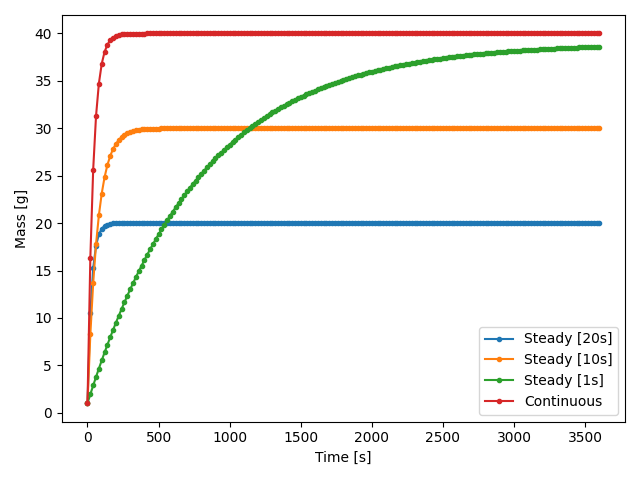
\includegraphics[scale=0.7]{images/dirlin-steady-comp.png}
  \caption{Plot comparing the values of continuous and batchwise reprocessing methods with a 40 second cycle time for an arbitrary nuclide.}
   \label{fig:steady_cont_repr_diff}
\end{figure}


It can be seen in this figure that the Direct Linear continuous method will result in a steady state result which is significantly different from the Steady batchwise method unless the depletion step size is infinitely small.

\begin{equation} \hfill
m_{ss} = \frac{C}{\lambda}
\hfill\label{eq:ss-mass-cont} \end{equation}

Equation \eqref{eq:ss-mass-cont} shows the steady state mass which will appear when using continuous reprocessing when there is a constant growth term. This can be set equal to the Steady batch steady state term in order to solve for the depletion time step needed to match the result from continuous reprocessing at steady state. The result of this can be seen in Equations \eqref{eq:ss-mass-solve-1} and \eqref{eq:ss-mass-solve-3}, which reinforces what can be seen in Figure \ref{fig:steady_cont_repr_diff}.

\begin{equation} \hfill
m_{ss}^{continuous} = \lim_{\Delta t \to 0} \left( m_{ss}^{batch} \right)
\hfill\label{eq:ss-mass-solve-1} \end{equation}

\begin{equation} \hfill
\frac{C}{\lambda} = \lim_{\Delta t \to 0} \left( \frac{C (e^{(\lambda - \lambda_r) \Delta t} - 1)}{\lambda - \lambda_r}  \left( \frac{\eta}{1 - \eta} \right) \right)
\hfill\label{eq:ss-mass-solve-3} \end{equation}

Correspondingly, this means that the steady state error associated with implementing the Steady batchwise method to approximate a continuous reprocessing scheme is directly proportional to the magnitude of the depletion step size used. Specifically, as shown in Equations \eqref{eq:ss-err-1} and \eqref{eq:ss-err-4}, the error at steady state due to reprocessing directly scales based on the ratio of the depletion time step and the cycle time.

\begin{equation} \hfill
|E| = \frac{|m_{ss}^{batch} - m_{ss}^{continuous}|}{m_{ss}^{continuous}}
\hfill\label{eq:ss-err-1} \end{equation}

%\begin{equation} \hfill
%|E| = \frac{|C(T_{cyc} - \Delta t) - CT_{cyc}|}{CT_{cyc}}
%\hfill\label{eq:ss-err-2} \end{equation}

%\begin{equation} \hfill
%|E| = \frac{|T_{cyc} - \Delta t - T_{cyc}|}{T_{cyc}}
%\hfill\label{eq:ss-err-3} \end{equation}

\begin{equation} \hfill
|E| = \frac{\lambda}{C} \left| \frac{C}{\lambda}  - \frac{\lambda (e^{(\lambda - \lambda_r) \Delta t} - 1)}{\lambda - \lambda_r}  \left( \frac{(1 - \lambda_r \Delta t) e^{-(\lambda - \lambda_r) \Delta t}}{1 - (1 - \lambda_r \Delta t) e^{-(\lambda - \lambda_r) \Delta t}} \right) \right|
%|E| = \frac{\Delta t}{T_{cyc}} \ni 0 < \frac{\Delta t}{T_{cyc}} \leq 1
\hfill\label{eq:ss-err-4} \end{equation}

This relative error can be seen in Figure \ref{fig:steady_cont_repr_diff}, as the depletion time step to cycle time ratio is exactly 2, and the steady state value is twice is low as the continuous steady state value. Although these equations show only the simplest case of a constant growth, they demonstrate how the important using a small depletion step size is for batchwise methods to generate an accurate result.

Although this example does not seem to apply to the more complicated interactions which are present in the molten salt reactor model, it actually fits closely. As previosuly discussed, by assuming there is a constant amount of fissile mass in the system, in the case of the MSBR this is primarily uranium-233, $m_{u233}$; the fission yield does not change due to spectral changes, $\gamma$; and a constant neutron flux, $\phi$; the equations can be expanded using the variables shown in Equation \eqref{eq:ss-mass-p5-update} and \eqref{eq:ss-mass-p5-steady-update}. The terms in these equations come from the Bateman equation.

\begin{equation} \hfill
C_i = \phi \sigma_{u233} \gamma N_{u233} + \sum_j N_j \left( \lambda_{j \rightarrow i }  + \sigma_{j \rightarrow i} \phi \right)
%\frac{dm}{dt} = \phi \sigma_{u233} \gamma m_{u233} - \left( \lambda_{r} + \lambda_d + \phi \sigma \right) m
\hfill\label{eq:ss-mass-p5-update} \end{equation}

\begin{equation} \hfill
\lambda_i = N_i \left( \lambda_{i, d} + \lambda_{i, r} + \sigma_i \phi \right)
%m_{n+1} = (m_n + \phi \sigma_{u233} \gamma m_{u233} \Delta t) (1 - \Delta t \left(  \lambda_{r} + \lambda_d + \phi \sigma \right) )
\hfill\label{eq:ss-mass-p5-steady-update} \end{equation}

In these equations, the reprocessing constant, $\lambda_r$, is rewritten from its previous form of $\lambda$ because the decay constant, $\lambda_d$, is now present.
Due to the simple assumptions made, which are valid over a short net depletion time or at steady state, these equations is of the same form as the simple equation presented in the example above.
Thus, by replacing the $C$ and $\lambda$ terms, the previous example provides a reasonable estimate of many isotopes in the reactor simulation.
This means that the error equation generated in Equation \eqref{eq:ss-err-4} remains reasonable for many fission product isotopes generated in the reactor at steady state.
%but for clarity could be rewritten in the form shown in Equation \eqref{eq:ss-err-4-final}.

%\begin{equation} \hfill
%|E| = \Delta t \lambda \ni 0 < \Delta t \lambda \leq 1
%\hfill\label{eq:ss-err-4-final} \end{equation}

%If the cycle time, instead of removing 100\%, removes some fraction $f$, then the equation can be modified using Equation \eqref{eq:batchwise_rem_eff-new} in order to get Equation \eqref{eq:ss-err-4-final-new}.

%\begin{equation} \hfill
%\gamma = f \frac{\Delta t}{T_{cyc}}
%\hfill\label{eq:batchwise_rem_eff-new} \end{equation}

%\begin{equation} \hfill
%|E| = f \Delta t \lambda \ni 0 < \Delta t \lambda \leq 1
%\hfill\label{eq:ss-err-4-final-new} \end{equation}

%Checking the limits, if the removal fraction $f$ is zero, then the continuous and batchwise methods should both remove nothing and therefore be equivalent. Additionally, when removing smaller fractions, it is expected that the amount of error possible for the batchwise method should be reduced, which also fits with the equation.

\paragraph*{Computational Cost}

One of the weaknesses of batchwise methods is the necessarily higher computational cost compared to continuous methods. The first reason for this is because batchwise methods which approximate a continuous process have reprocessing based error which scales with depletion step size, as shown in Equation \eqref{eq:ss-err-4}. This means that smaller depletion step sizes are required for the same error as a continuous method.

The second reason is because of the "double-running" of simulations which is required when using a batchwise method in Serpent2. When running a batchwise depletion program, the first time step is run and the new material compositions are generated, providing 2 complete simulation results at times 0 and $\Delta t$. However, these generated materials do not have reprocessing factored in, so the external reprocessing script, such as SaltProc, then performs the reprocessing on the materials. The updated materials are fed back in, and the simulation is run again. This results in two new simulation results at $\Delta t$ and $2 \Delta t$.

Because of the necessity of regenerating data based on the updated material properties after the external depletion is performed, each time step requires two simulations to be performed, essentially doubling the computational cost. With a continuous method, the materials are updated during the depletion step, which means the generated data already uses the data of reprocessing materials. This eliminates any need for double running, allowing continuous methods to be run for much less computational cost.

\section{Continuous Reprocessing}

The continuous reprocessing functionality of Serpent2 was originally sparsely documented on user forums, but as of October 2020, more comprehensive documentation has been made available \cite{seifert_material_2020}.
However, there has not been comparisons of Serpent2 continuous reprocessing with Serpent2 batchwise reprocessing with no differences between the models aside from the mathematical reprocessing approach used.

There are three different options which can be used for the Serpent2 built-in continuous reprocessing. The different options are defined in Serpent2 as 0, 1, and 2; which are henceforth referenced as Constant, Decay, and Step reprocessing. These names are selected because they closely describe the behaviour of each of the methods.

\subsection{Constant}
The Constant reprocessing method is the only method of the three options which does not conserve mass. This option instead generates mass the same way as the Decay reprocessing method for the initial step, then continues using that mass rate from that point onwards.

This method is useful for handling a constant fresh fuel feed rate, or any other situation where a constant addition of mass is desired. Because this method does not remove mass, it is not useful for any sort of constant removal.
%The main issue with this method is that it, for Serpent 2.32.1, it causes depletion to cease functioning while this method is active. This is an issue, since for most cases where a user wants to incorporate a feed rate, depletion is being considered.

\subsection{Decay}
The Decay reprocessing method is the most useful of the three options, and that is due to its flexibility in its usefulness. This method adds a decay term to whatever material it is attached to, and that decay term becomes a feed term to whatever material is set to receive the flow. For fission product removal, this is likely some material which is not modeled in the geometry of the problem but only exists to receive the fission product waste. However, this term can instead be leveraged to turn it into a feed rate.

This can be performed by attaching the decay term to a material which contains a volume of the desired feed, and then having that material feed into the core. The feed then "decays" from the feed tank into the core, essentially operating as a feed. Using this same method but altering the reprocessing constant or volume of the feed tank allows for an essentially constant feed rate, where the removed mass is negligible compared to the net mass.

Additionally, for this method, there are multiple approaches which can be used to calculate the reprocessing constants that should be implemented. These approaches are named "Cycle Time Decay", "Cycle Rate", and "SaltProc Cycle Rate" accordingly. The Cycle Time Decay approach treats the cycle time as if it is twice a half-life, and the cycle time is an exponential process. The Cycle Rate approach treats the cycle time as the time where 100\% of removal occurs, and then linearly extrapolates by assuming an equal percentage removal occurs up to that point.

The reason these approaches are implemented is because molten salt reactor reprocessing schemes provide reprocessing data in terms of cycle times. The cycle time is the amount of time it takes for a given element to be removed from the system. This cannot be directly solved using the Bateman equation, as shown in Equations \eqref{eq:decay_1} through \eqref{eq:decay_3} and \eqref{eq:decay_4} through \eqref{eq:decay_7}.

\begin{equation} \hfill
\frac{dN}{dt} = -\lambda_r N
\hfill\label{eq:decay_1} \end{equation}

\begin{equation} \hfill
N(\Delta t) = 0 = N_0 e^{-\lambda_r \Delta t}
\hfill\label{eq:decay_2} \end{equation}

\begin{equation} \hfill
-ln(0) = \lambda_r \Delta t
\hfill\label{eq:decay_3} \end{equation}

Equations \eqref{eq:decay_1} through \eqref{eq:decay_3} show how the solution results in a reprocessing constant of infinity when only continuous removal is considered.

\begin{equation} \hfill
\frac{dN}{dt} = C -\lambda_r N
\hfill\label{eq:decay_4} \end{equation}

\begin{equation} \hfill
N(\Delta t) = 0 = N_0 e^{-\lambda_r \Delta t} + \frac{C}{\lambda_r} \left( 1 - e^{-\lambda_r \Delta t} \right)
\hfill\label{eq:decay_5} \end{equation}

\begin{equation} \hfill
0 = N_0 e^{-\lambda_r \Delta t} + \frac{C}{\lambda_r} - \frac{C}{\lambda_r} e^{-\lambda_r \Delta t}
\hfill\label{eq:decay_6} \end{equation}

\begin{equation} \hfill
0 = \lambda_r N_0 e^{-\lambda_r \Delta t} + C - C e^{-\lambda_r \Delta t}
\hfill\label{eq:decay_7} \end{equation}


 Equations \eqref{eq:decay_4} through \eqref{eq:decay_7} show that the only real solution to a steady accumulation and continuous removal is with a reprocessing constant of 0.

\subsubsection{Cycle Time Decay}
\label{s:CTD}

The Cycle Time Decay approach is a simple method which makes use of the mathematical form of the Decay reprocessing method. A similar method of treating removal periods for reprocessing can be seen in Brovchenko et al \cite{brovchenko_neutronic_2019}. Because it adds a "decay-like" term to the Bateman equation, this approach takes the cycle time for the target, cuts it in half, and then treats that value as the reprocessing half-life for that target. This process is shown in Equations \eqref{eq:ctd_1} and \eqref{eq:ctd_2}.

\begin{equation} \hfill
\Delta t_{1/2} = \frac{T_{cyc}}{2}
\hfill\label{eq:ctd_1} \end{equation}

\begin{equation} \hfill
\lambda_r = \frac{ln(2)}{\Delta t_{1/2}}
\hfill\label{eq:ctd_2} \end{equation}

%An example of how this approach is mathematically modeled can be seen in Figure \ref{fig:ctd_examp}.

%\begin{figure}[H]
%  \centering
%  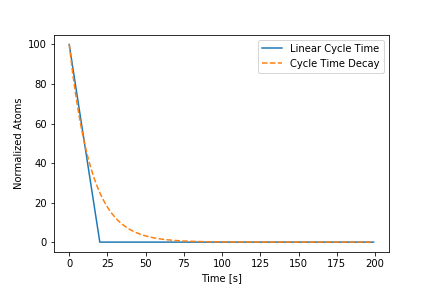
\includegraphics[scale=0.6]{images/Cycle_Time_Decay_example_0.png}
%  \caption{A comparison between a linear 20 second cycle time and the Cycle Time Decay approach.}
%   \label{fig:ctd_examp}
%\end{figure}

%It can be seen in this figure that this approach is accurate in being close to the cycle time, though this accuracy is limited to above approximately 40\% of the atoms. Because fission products are continuously generated though, it is expected to be within the more accurate regions.
%Figure \ref{fig:ctd_examples} shows how the Cycle Time Decay approach fares when accumulation of fission products is incorporated into the problem.

%\begin{figure}[H]
%  \centering
%  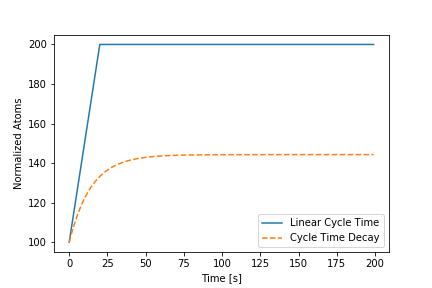
\includegraphics[scale=0.6]{images/Cycle_Time_Decay_example_10.png}
%  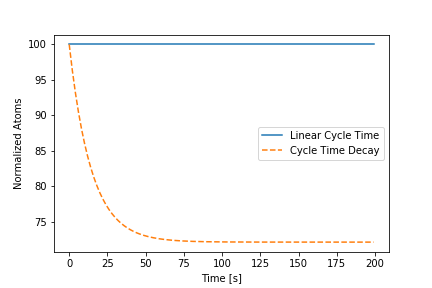
\includegraphics[scale=0.6]{images/Cycle_Time_Decay_example_5.png}
%  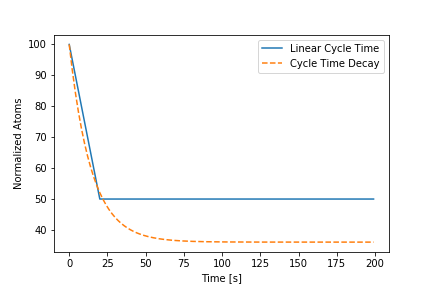
\includegraphics[scale=0.6]{images/Cycle_Time_Decay_example_2.5.png}
%  \caption{Comparison with linear 20 second cycle time and Cycle Time Decay approach for 10, 5, and 2.5 %atoms per second accumulation, respectively.}
%   \label{fig:ctd_examples}
%\end{figure}

%The top plot of Figure \ref{fig:ctd_examples} shows a situation where the accumulation of fission products occurs at a higher rate than the cycle time, leading to a larger steady-state value than initially present. The Cycle Time Decay does not reach the 200 value and instead is lower at 144. The middle plot shows a situation where the accumulation rate matches the cycle time removal rate, the same rate that the linear cycle time would have them removed, resulting in a steady-state value. However, the Cycle Time Decay approach drops to approximately 72 levels off. The bottom plot shows an accumulation which is half the linear cycle time removal rate. These results are somewhat close, though the Cycle Time Decay does not reach the same steady-state value, instead stabilizing around 40 instead of 50. For various accumulation rates ranging from 0.1 to 1 million atoms per second, the steady-state difference comes out to approximately 27.86\% for each. This percent difference also stays the same for different cycle times as well.

An example of implementing this approach for a 30 second cycle time would then have a 15 second reprocessing half-life. This is then converted to a reprocessing constant in the same way that a decay half-life is converted to a decay constant, which can be seen in Equation \eqref{eq:ctd_eqn}, resulting in a value of 0.0462 $s^{-1}$.

\begin{equation} \hfill
\lambda_{r} = \frac{ln(2)}{15} = 0.0462 s^{-1}
\hfill\label{eq:ctd_eqn} \end{equation}

\subsubsection{SaltProc Cycle Time Decay}

This approach is the same as Cycle Time Decay, but alters for any target which has a cycle time less than the batchwise reprocessing step incorporated by SaltProc. For example, a 3 day cycle time for some target would be treated the same as the standard Cycle Time Decay. However, a cycle time shorter than the 3 day batchwise reprocessing step used by SaltProc for the MSBR has its half-life extended to the SaltProc minimum value of 1.5 days. For example, a 30 second cycle time would instead be treated as a 3 day cycle time, which would result in a half-life of 1.5 days. Plugging in, this would result in a reprocessing constant of 0.462 $days^{-1}$, or 5.348E-6 $s^{-1}$. This is the reprocessing constant for any cycle time which is less than or equal to three days. Additionally, the decay constant is multiplied by the fractional efficiency of the removal used by SaltProc. In most cases the value is 1, but it is roughly 0.91 for xenon and krypton.

\subsubsection{Cycle Rate}
\label{s:CR}

The Cycle Rate approach uses a linear approximation such that the inverse of the cycle time is the rate at which material is removed. This is represented by, for example, 10\% removal per second would neglect the efficiency decrease over time and give 100\% removal after 10 seconds. This is calculated by investigating a unit time progression, i.e. 1 second or 1 day. Over this time period, the removal of atoms should be the fractional rate value, which means the final atom count at a time of 1 should be 1 - $f$, where $f$ is the fractional removal rate. This can be seen in Equations \eqref{eq:nat_log_0} and \eqref{eq:nat_log_3}.

\begin{equation} \hfill
f = \frac{1}{T_{cyc}}
\hfill\label{eq:nat_log_0} \end{equation}

\begin{equation} \hfill
\frac{dN}{dt} = -\lambda_r N
\hfill\label{eq:nat_log_1} \end{equation}

\begin{equation} \hfill
N(t) = N_0 e^{-\lambda_r t}
\hfill\label{eq:nat_log_1_half} \end{equation}

\begin{equation} \hfill
N(t = 1) = (1-f) N_{0}
\hfill\label{eq:nat_log_2} \end{equation}

\begin{equation} \hfill
(1-f) N_{0} = N_{0} e^{-\lambda_r (1)}
\hfill\label{eq:nat_log_2_1} \end{equation}

\begin{equation} \hfill
-ln(1-f)  = \lambda_r
\hfill\label{eq:nat_log_2_5} \end{equation}

\begin{equation} \hfill
\lambda_r = ln\left( \frac{1}{1-f} \right)
\hfill\label{eq:nat_log_3} \end{equation}

%However, the mathematical model actually results in exponential decay in the removal effectiveness due to a decreasing amount of the target to remove. %Figure \ref{fig:cr_examp} shows how this approach compares to the actual exponential decay.

%\begin{figure}[H]
%  \centering
%  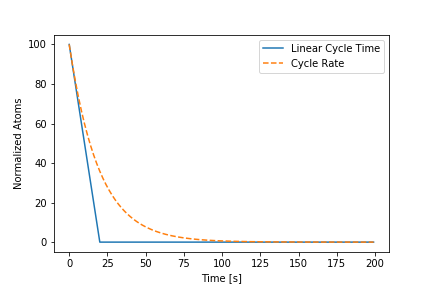
\includegraphics[scale=0.6]{images/Cycle_Rate_example_0.png}
%  \caption{A comparison between a linear 20 second cycle time and the Cycle Rate approach.}
%   \label{fig:cr_examp}
%\end{figure}

%It can be seen from this figure that the Cycle Rate approach removes at a rate sufficient to match the cycle time of 20 seconds while there are ~60\% of the atoms present. Once the atom count drops, the removal becomes less effective however, which is physical but makes the model less effective at matching the cycle time. Because the Cycle Rate approach is used on fission products which are being constantly generated, the difference is expected to be fairly small.

%\begin{figure}[H]
%  \centering
%  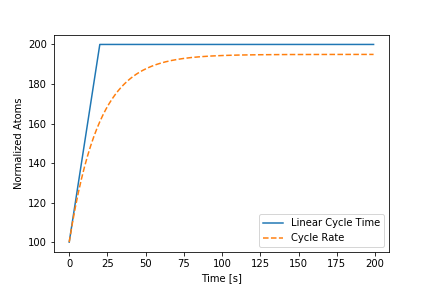
\includegraphics[scale=0.6]{images/Cycle_Rate_example_10.png}
%  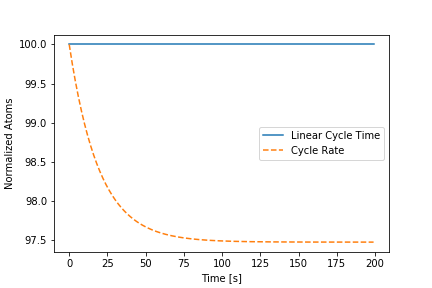
\includegraphics[scale=0.6]{images/Cycle_Rate_example_5.png}
%  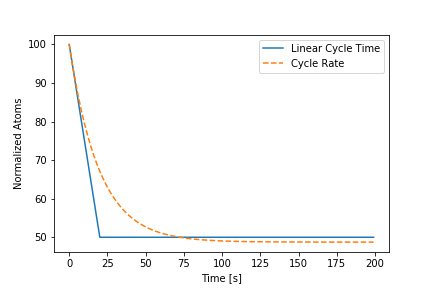
\includegraphics[scale=0.6]{images/Cycle_Rate_example_2.5.png}
%  \caption{Comparison with linear 20 second cycle time and Cycle Rate approach for 10, 5, and 2.5 atoms %per second accumulation, respectively.}
%   \label{fig:cr_examples}
%\end{figure}



An example cycle time of 30 seconds would be modeled by taking the inverse, which gives 0.033 $s^{-1}$. This value is then converted to a reprocessing constant by plugging it into the solved differential equation form shown in Equations \eqref{eq:cr_exmp1} and \eqref{eq:cr_eqn}, giving a value of 0.0339 $s^{-1}$.

\begin{equation} \hfill
f = \frac{1}{30} = 3.33E\minus2 s^{-1}
\hfill\label{eq:cr_exmp1} \end{equation}

\begin{equation} \hfill
\lambda_{r} = ln\left(\frac{1}{1 - 3.33E\minus2}\right) = 0.0339 s^{-1}
\hfill\label{eq:cr_eqn} \end{equation}

%The reason this approach is used is two-fold. Firstly, SaltProc v0.3 uses the same linear fractional removal approximation for its batchwise removal, so this same method is employed to better compare the two models. Secondly, due to the mathematical nature of the Decay reprocessing model, 100\% removal only occurs for a reprocessing constant of infinity. This means an approximation must be made. This is also a reasonable approximation since there is constant addition of material, meaning that the exponential line and the linear line are not going to be significantly different.


\subsubsection{SaltProc Cycle Rate}

The SaltProc Cycle Rate approach is the same as the Cycle Rate approach, but takes into account the limiting nature of the 3 day batchwise reprocessing step used by SaltProc. For example, a 6 day cycle time target would be modeled the same using the SaltProc Cycle Rate approach as the standard Cycle Rate approach. However, anything shorter than 3 days would be modeled differently, since that is the batchwise reprocessing step inocorporated by SaltProc for modeling the MSBR. For example, a 30 second cycle time would be analyzed instead as a 3 day cycle time, since SaltProc can only remove 100\% of material after a minimum of 3 days. This means the inverse would be 0.333 $days^{-1}$, or 3.858E-4 $s^{-1}$. Converting to a reprocessing constant gives a value of 3.858E-6 $s^{-1}$. This is the reprocessing constant for any cycle time which is less than or equal to three days. Additionally, the decay constant is multiplied by the fractional efficiency of the removal used by SaltProc. In most cases the value is 1, but it is roughly 0.91 for xenon and krypton.

\subsubsection{Direct Linear Approach}
\label{s:DL}

Another approach is to directly apply the Cycle Rate removal rate, which is the inverse of the cycle time, as the reprocessing constant \cite{hombourger_eql0d_2020}. This is referred to as the Direct Linear approach. This approach is similar to the Cycle Rate approach, though the derivation for it is slightly different. This can be seen in Equations \eqref{eq:dir_lin_0} through \eqref{eq:dir_lin_10}, where Equations \eqref{eq:dir_lin_8} and \eqref{eq:dir_lin_9} uses L'Hôpital's rule.

\begin{equation} \hfill
f = \frac{1}{T_{cyc}}
\hfill\label{eq:dir_lin_0} \end{equation}

\begin{equation} \hfill
\frac{dN}{dt} = -\lambda_r N
\hfill\label{eq:dir_lin_1} \end{equation}

\begin{equation} \hfill
N(t) = N_0 e^{-\lambda_r t}
\hfill\label{eq:dir_lin_1_2} \end{equation}

\begin{equation} \hfill
N_{cur} = N_{prev} e^{-\lambda_r \Delta t}
\hfill\label{eq:dir_lin_2} \end{equation}

\begin{equation} \hfill
N_{cur} = (1 - \Delta t f) N_{prev}
\hfill\label{eq:dir_lin_3} \end{equation}

\begin{equation} \hfill
(1 - \Delta t f) N_{prev} = N_{prev} e^{-\lambda_r \Delta t}
\hfill\label{eq:dir_lin_4} \end{equation}

\begin{equation} \hfill
-ln\left((1 - \Delta t f)\right) = \lambda_r \Delta t
\hfill\label{eq:dir_lin_5} \end{equation}

\begin{equation} \hfill
\lambda_r = \frac{-ln\left((1 - \Delta t f)\right)}{\Delta t}
\hfill\label{eq:dir_lin_6} \end{equation}

\begin{equation} \hfill
\lambda_r = lim_{\Delta t \to 0} \frac{-ln\left((1 - \Delta t f)\right)}{\Delta t}
\hfill\label{eq:dir_lin_7} \end{equation}

\begin{equation} \hfill
\lambda_r = \frac{0}{0}
\hfill\label{eq:dir_lin_8} \end{equation}

\begin{equation} \hfill
\lambda_r = lim_{\Delta t \to 0} \frac{f}{1-f\Delta t}
\hfill\label{eq:dir_lin_9} \end{equation}

\begin{equation} \hfill
\lambda_r = f = \frac{1}{T_{cyc}}
\hfill\label{eq:dir_lin_10} \end{equation}

These equations follow a similar path to the Cycle Rate approach, but instead of using the linear approximation value after a unit time step, this approach generates the reprocessing constant while implementing the linear approximation as the time step goes to zero.

The differences between Cycle Rate and Direct Linear approaches can be seen in Table \ref{tab:repr_decay_view}, where for longer cycle times, the difference is negligible, but for shorter cycle times, the difference becomes larger. However, since extremely short cycle times are not realistically practical, the two approaches are approximately equivalent. Overall, the Direct Linear approach is more numerically stable, however, since it does not have asymptotic until reaching a cycle time of 0 seconds, whereas the Cycle Rate method has asymptotic behaviour at 1 second cycle time. This can be seen in Figure \ref{fig:dl_cr_asymptotic}. The asymptotic behaviour for a 0 second cycle time is not an issue because there are no negative cycle times, meaning the value is only approached from the positive side and behaves as physically expected.

\begin{table}[H]
\renewcommand{\arraystretch}{1.25}
\caption{Subset of Decay Reprocessing Approaches}
\label{tab:repr_decay_view}
\begin{center}
\begin{tabular}{ c | c | c | c | c }
 \hline
 Cycle Time & Removal Rate [$s^{-1}$] & CR $\lambda_{r}$ [$s^{-1}$] & DL $\lambda_{r}$ [$s^{-1}$] & $\Delta \lambda_{r}$\\
 \hline
 \hline
 3 d & 3.86E-6 & 3.86E-6 & 3.86E-6 & 7.44E-12\\
 20 s & 0.05 & 5.13E-2 & 5.00E-2 & 1.29E-3\\
 5 s & 0.2 & 2.23E-1 & 2.00E-1 & 2.31E-2\\
 2 s & 0.5 & 6.93E-1 & 5.00E-1 & 1.93E-1\\
 1 s & 1 & - & 1 & -\\
 \hline
\end{tabular}
\end{center}
\end{table}

\begin{figure}[H]
  \centering
  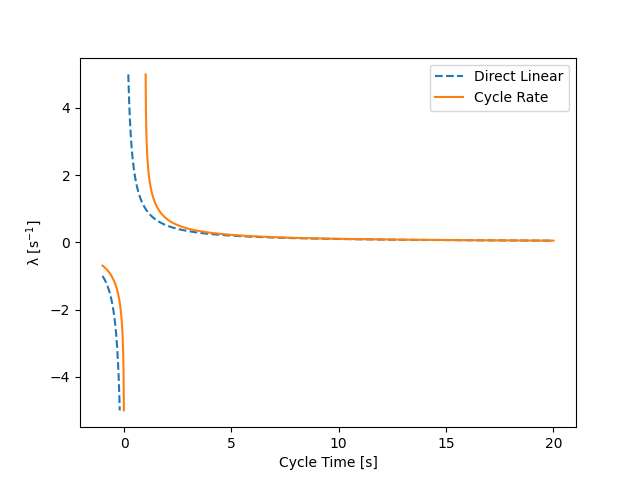
\includegraphics[scale=0.55]{images/dl_cr_asymptote.png}
  \caption{A comparison of the Direct Linear and Cycle Rate reprocessing constants for different cycle times.}
   \label{fig:dl_cr_asymptotic}
\end{figure}

Because the shortest cycle time for the MSBR is 20 seconds, this shows that the Cycle Rate and Directly Linear approaches are roughly equivalent for this reprocessing scheme.

%Figure \ref{fig:dl_cr_compare_linear} shows the implementation of both methods for an example nuclide with a cycle time of CYCLE TIME and an accumulation rate of ACCUMULATION RATE. It can be seen from this figure how the Direct Linear and Cycle Rate approaches differ in modeling of the same isotope.

%\begin{figure}[H]
%  \centering
%  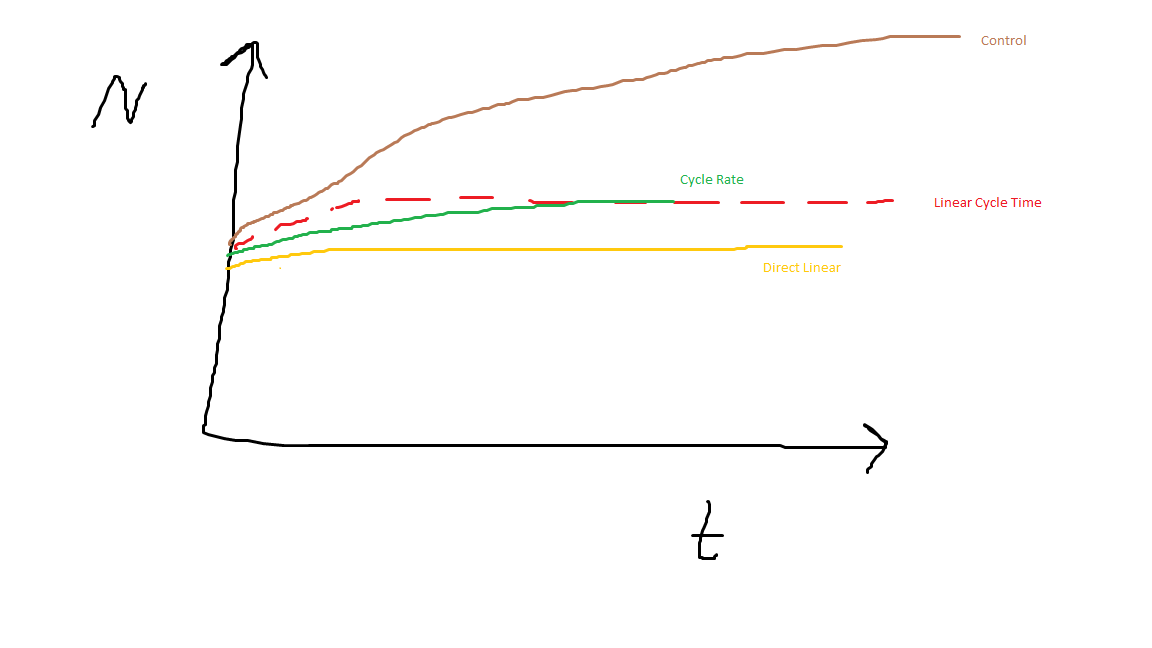
\includegraphics[scale=0.25]{images/direct_linear_compare.png}
%  \caption{A comparison of the Direct Linear and Cycle Rate approaches for a particular element with a %given accumulation rate and cycle time(s).}
%   \label{fig:dl_cr_compare_linear}
%\end{figure}

\subsubsection{SaltProc Direct Linear Approach}

The SaltProc Direct Linear approach follows the same trend as the other SaltProc-based modified approaches. This includes changing the smallest time scale to 3 days and altering the fractional removal values of xenon and krypton.

\subsubsection{Decay Approaches Summary}

Figure \ref{fig:repr_cnst} shows how the reprocessing constants for the different approaches vary as a function of cycle time.

\begin{figure}[H]
  \centering
  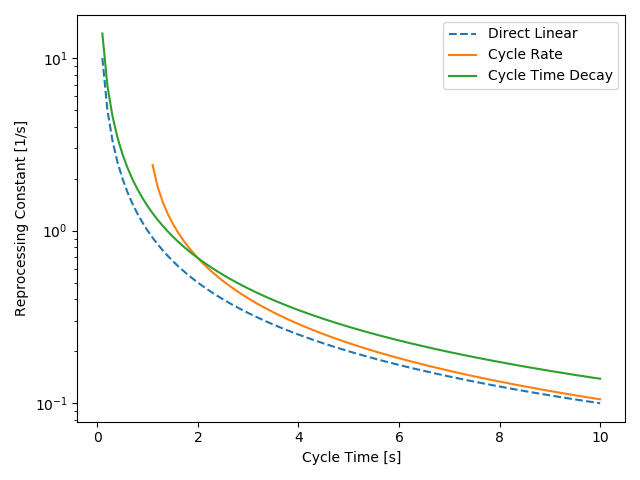
\includegraphics[scale=0.7]{images/cont-compare-cycles.png}
  \caption{Plot of how reprocessing constants for different approaches vary with cycle time.}
   \label{fig:repr_cnst}
\end{figure}

Figure \ref{fig:repr_cnst} shows the three different continuous decay based methods for reprocessing as a function of various cycle times. From the figure, it can be seen that the Cycle Rate method does not have results for cycle times less than or equal to 1 second, which is a significant weakness of the method since physical processes could exist with a cycle time in that range. The other two methods provide results down to a 0 second cycle time, which allows full coverage of possible cycle time values.

The Direct Linear method behaves similarly to the Cycle Time Decay method during small cycle times and the Cycle Rate method for longer cycle times. This is due to the general form of the equations for each, where at small cycle times the inverse cycle time relationship with the Cycle Time Decay method dominates, while at larger cycle times the Cycle Rate log of the inverse term matches more closely.


Table \ref{tab:repr_decay_view_full} shows all the different decay based continuous reprocessing approaches for various cycle times. From this table, it can be seen that the Direct Linear and Cycle Rate methods are very close, while the Cycle Time Decay method is off by a small amount at all cycle times. In terms of the SaltProc variants, the main difference is the fact that the cycle times below three days have been assigned the reprocessing constant of the three day cycle time.

\begin{table}[H]
\renewcommand{\arraystretch}{1.25}
\caption{Full Set of Decay Reprocessing Approaches for Various Cycle Times}
\label{tab:repr_decay_view_full}
\begin{center}
\begin{tabular}{ c | c | c | c | c }
 \hline
 Method & $T_{cyc} = 1 s$ & $T_{cyc} = 20 s$ & $T_{cyc} = 3 d$ & $T_{cyc} = 50 d$\\
 \hline
 \hline
 DL & 1 & 5.00E-2 & 3.86E-6 & 2.31E-7\\
 CR & - & 5.13E-2 & 3.86E-6 & 2.31E-7\\
 CTD & 1.39 & 6.93E-2 & 5.35E-6 & 3.21E-7\\
 \hline
 SPDL & 3.86E-6 & 3.86E-6 & 3.86E-6 & 2.31E-7\\
 SPCR & 3.86E-6 & 3.86E-6 & 3.86E-6 & 2.31E-7\\
 SPCTD & 5.35E-6 & 5.35E-6 & 5.35E-6 & 3.21E-7\\
 \hline
\end{tabular}
\end{center}
\end{table}

The values shown in Table \ref{tab:repr_decay_view_full} for the SaltProc-type continuous methods are based on the cycle times given from the Robertson report, which matches what is used in the Bulk SaltProc, version 0.1, results. The Steady SaltProc results, verson 0.3, do not use these exact values \cite{robertson_conceptual_1971, rykhlevskii_advanced_2018}. The differences in Steady SaltProc are as follows: xenon has 91.2\% removal over three days instead of 100\%, krypton has 91.5\% removal over three days instead of 100\%, protactinium has 9.5\% removal over three days instead of 100\%, and the discard has a removal of 0.9\% over three days instead of 0.09\%. %Check Pa, SaltProc actually using 9.5%?????????

%WHICH IS THE MORE ACCURATE APPROACH AMONG THE THREE (There isn't a way to validate this without more information on how cycle time is generated. Perhaps if instead we find data for molten salt reprocessing and compare against that it might be useful?) (Maybe check average net atoms for steady and bulk batch and compare, then maybe check a comparison of net atoms at 1/2 cycle time and cycle time, etc.)

%CITE "Liquid Fuel Molten Salt Reactors for Thorium Utilization" This paper uses bulk batchwise reprocessing

%INCLUDE PLOT OF N(t) FOR DIFFERENT CYCLE TIMES WHERE ONLY INITIAL MASS AND REPROCESSING ARE CONSIDERED. (Direct Linear AND Cycle Rate ARE THE SAME FOR LARGE CYCLE TIMES)

%REPLICATE ATOMS OVER TIME PLOTS FOR DIFFERENT MODELS AND DIFFERENT ACCUMULATION RATES TO SEE HOW STEADY-STATE VALUES COMPARE.

\subsection{Step}

The Step reprocessing method implemented in Serpent2 is mathematically very similar to the Decay model, but instead of updating continuously in time, it instead is updated during new depletion steps. In this manner, it is a sort of mix between the Constant method and the Decay method. This is because over a single depletion step, it is a constant added or subtracted from the Bateman equation, while over many depletion steps, it follows the same exponential decay form of the Decay method.

This particular method is not useful for extracting fission products, and is not needed for constant feed rates since that can be modeled using the Decay method. This method could be useful for inducing a step drop in feed rate, though this would require running only a single depletion step until the drop occurred. Additionally, this drop could be simulated by running the Decay method and reducing the reprocessing constant. This would allow for flexibility in the distribution of depletion steps as well without having to worry about changing the behaviour of the reprocessing functionality.

Another potential issue with the Step method is that the depletion step can last long enough that the constant mass removal causes the mass to go negative. However, Serpent2 will cease running if this occurs. The Decay method does not mathematically allow for negative mass, the Constant method does not conserve mass, and the Step method stops running once there is negative mass.

The main potential use of the Step reprocessing may be for movement of material at a set rate. This could be implemented by writing a script to check the current number of atoms of the target and adjusting the reprocessing rate accordingly. However, for the MSBR, this form of reprocessing is not necessary, and is thus not implemented.

\section{Mass Balancing}

One of the useful features of batchwise reprocessing is that the net mass of the core can be balanced by adjusting the feed rates to provide the same amount into the core that is removed through reprocessing. Alternative methods also exist, such as removing excess mass or increasing the volume \cite{ridley_method_2017}. SaltProc version 0.1 does not account for mass balancing but maintains a constant thorium mass, whereas SaltProc version 0.3 has the feed rates set to maintain mass. Mass balancing is particularly important in Serpent2 due to the way masses in Serpent2 are handled.

In Serpent2, an increase in mass does not affect volume, but instead increases the density of that isotope in the material accordingly. This affects macroscopic cross section calculations, and can lead to variation in results if not accounted for, since in reality volumetric expansion could be assumed. Though there are several methods to handle mass balancing with a batch method, it not currently continuously possible in Serpent2.

In order to balance the mass in Serpent2 continuously, one approach could be to iteratively perform depletion calculations while updating feed rates until a balanced mass is found while also minimizing some other parameter, such as net mass of material added. However, the current reprocessing options available in Serpent2 only allows for pseudo-constant and decaying feed rates over the depletion step. With those two feed types available, it is not possible to have a constant mass balance.

It is possible to have the masses at the end of each depletion step remain constant, but this does handle mass fluctuations during depletion. It does, however, solve the issue of the density variation causing a difference in cross sections.

Overall, if the net mass difference is sufficiently small, it does not have to be considered since the results would not be significantly impacted. To check this for the MSBR, a simple back-of-the-envelope calculation can be used. To determine the maximum possible increase in density, the mass loss due to fission and reprocessing is neglected, and only mass addition from the thorium feed rate is considered. The uranium feed is not added because it is equivalent to the protactinium removal, so it would have a negligible impact on net mass.

\begin{equation} \hfill
\Delta m = \Dot{m}_{feed} \Delta t \approx (2.5)(6000) = 15,000 kg
\hfill\label{eq:m_gain} \end{equation}

It can be seen in Equation \eqref{eq:m_gain} that the net mass gain for an average feed rate of 2.5 kilograms per day over 6000 days is 15,000 kg \cite{rykhlevskii_fuel_2020, betzler_molten_2017}. This does seem to be a very large value, but the importance of the mass in the depletion calculation is primarily in how it affects cross sections, which means that the impact on the overall thorium density is important. The thorium density is 1.46 grams per cubic centimeter, and the net volume is approximately 48.71 cubic meters. The density with the added mass is calculated using Equation \eqref{eq:new_rho}.

\begin{equation} \hfill
\rho_f = \frac{m_0 + \Delta m}{V} = \frac{(4.871E7)(1.45919E\minus3) + (15,000)}{4.871E7}
\hfill\label{eq:new_rho} \end{equation}

The final density comes out to be 1.767 grams per cubic centimeter, which is a percent difference of ~21\%. Although this is an upper bound on the mass difference, a 21\% difference in the expected cross section would result in significant error in the results. Therefore, since it is possible for the mass balancing to have an impact, it should be investigated to ensure the mass balancing is not impacting the results in any unexpected manner.

%DIFFERENT FEED RATE VARIANTS IMPLEMENTED

%MSBR MASS BALANCE BATCH AND CONTINUOUS


%\section{Uncertainty}

%SHANNON ENTROPY

%STOCHASTIC ERROR VS ACTUAL DIFFERENCE IN RESULTS

%DEPLETION ERROR BUILDUP

%\section{Continuous Reprocessing Implementation}

\section{Effects of Delayed Neutrons on Depletion}

Delayed neutrons have a softer energy spectrum and drift along with the movement of the fuel salt in a fluid fueled molten salt reactor. This means that the delayed neutron precursors, of which some fraction leave the core and some move to less neutron important regions, have the potential to alter the depletion results of the MSBR model.

However, it has been shown by Zhou et al that for the MSBR, the delayed neutron precursor drift has a negligible impact on depletion results \cite{zhou_fuel_2018}. Although Zhou et al has shown this, it is still worth considering the maximum possible effect delayed neutron precursors could have on depletion results. In order to determine this, the Serpent2 functionality of disabling delayed neutrons is employed \cite{leppanen_serpent_2015}. Using this method, two different models are generated of the MSBR. The first is one in which the delayed neutron precursors are evenly distributed within the core, which is the model implemented by SaltProc and this work \cite{rykhlevskii_modeling_2019}. The second model is one in which delayed neutrons no longer exist. This is beyond the greatest effects the delayed neutron precursor drift could have on depletion, so the absolute maximum effect of delayed neutron precursors on depletion results can be determined.

Because the delayed neutron precursors are fission products or come from the decay of fission products, depletion must be performed. For reprocessing, the average feed rate from SaltProc is used with continuous Direct Linear reprocessing, while Direct Linear reprocessing is used for fission product removal.

The impact on $k_{eff}$ was investigated, and it was determined that the delayed neutrons from fission products add roughly 20 pcm to $k_{eff}$ after 6,000 days of operation, which is roughly steady state operation. The masses of various isotopes, such as uranium-235 and thorium-232, were also compared, though no statistically significant difference was found. Therefore, the net impact of delayed neutrons from fission product precursors is negligible on depletion results, which agrees with the results from Zhou et al.

%Figure \ref{fig:keff_compare} shows how the multiplication factors evolve over time. The final difference between the two values is FINALDIFF.

%\begin{figure}[H]
%  \centering
%  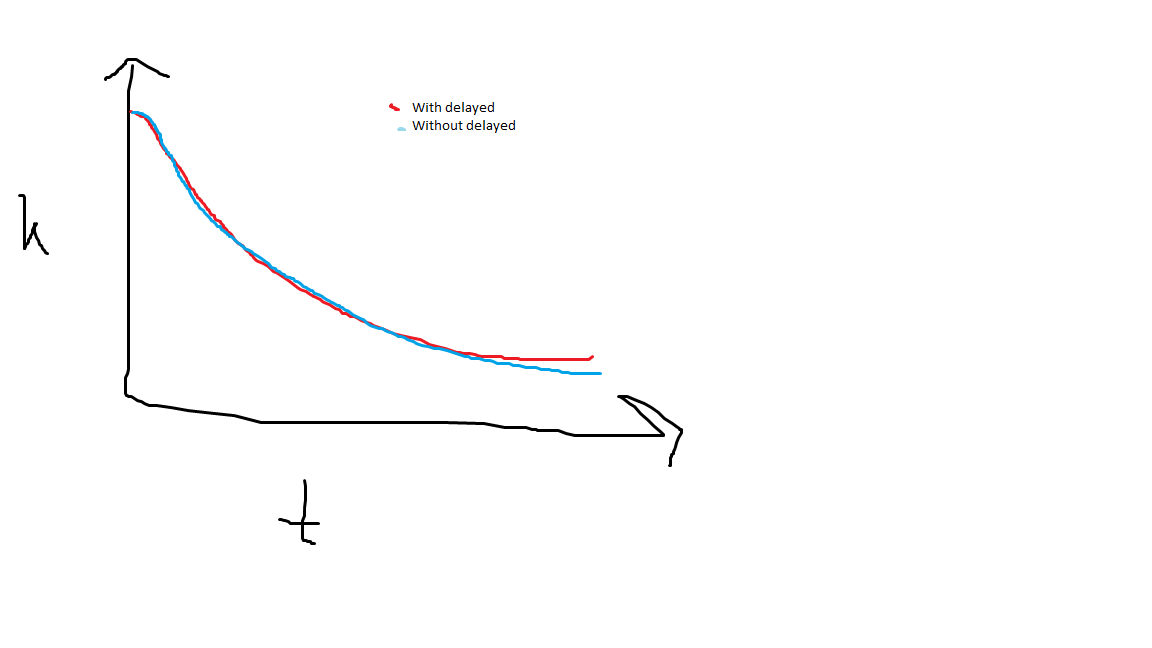
\includegraphics[scale=0.7]{images/keff_dnp_compare.png}
%  \caption{Comparison of $k_{eff}$ over time with and without delayed neutrons.}
%   \label{fig:keff_compare}
%\end{figure}

%PLOT OF SPECTRUMS WITH AND WITHOUT DELAYED NEUTRONS

%TABLE OF IMPORTANT ISOTOPE CONCENTRATIONS FOR WITH AND WITHOUT





% Toggle remove this for debugging
%\nocite{*}


\section{Serpent MSBR Model}

The results generated in this work come from the MSBR, particularly the model developed by Rykhlevskii \cite{rykhlevskii_advanced_2018}. The geometry of the model has remained unchanged, while the reprocessing has been overhauled using the continuous reprocessing functionality in Serpent2 which was previously undocumented. Previously, SaltProc's batchwise reprocessing was used, but the continuous reprocessing in Serpent2 is incorporated in this work.

\subsection{Reprocessing Structure}
\label{s:decay-tank}

There are two different reprocessing schemes developed in this work. Both schemes follow the MSBR reprocessing scheme, and vary how refueling functions. The first method matches the method of Rykhlevskii, where the uranium-233 feed is treated as equivalent to the protactinium-233 removal rate. In this case, the average uranium-233 feed rate from Rykhlevskii is used over the entire simulation time \cite{rykhlevskii_advanced_2018}. A simplified overview of this scheme can be seen in Figure \ref{fig:spmatchrepr}.


\begin{figure}[H]
  \centering
  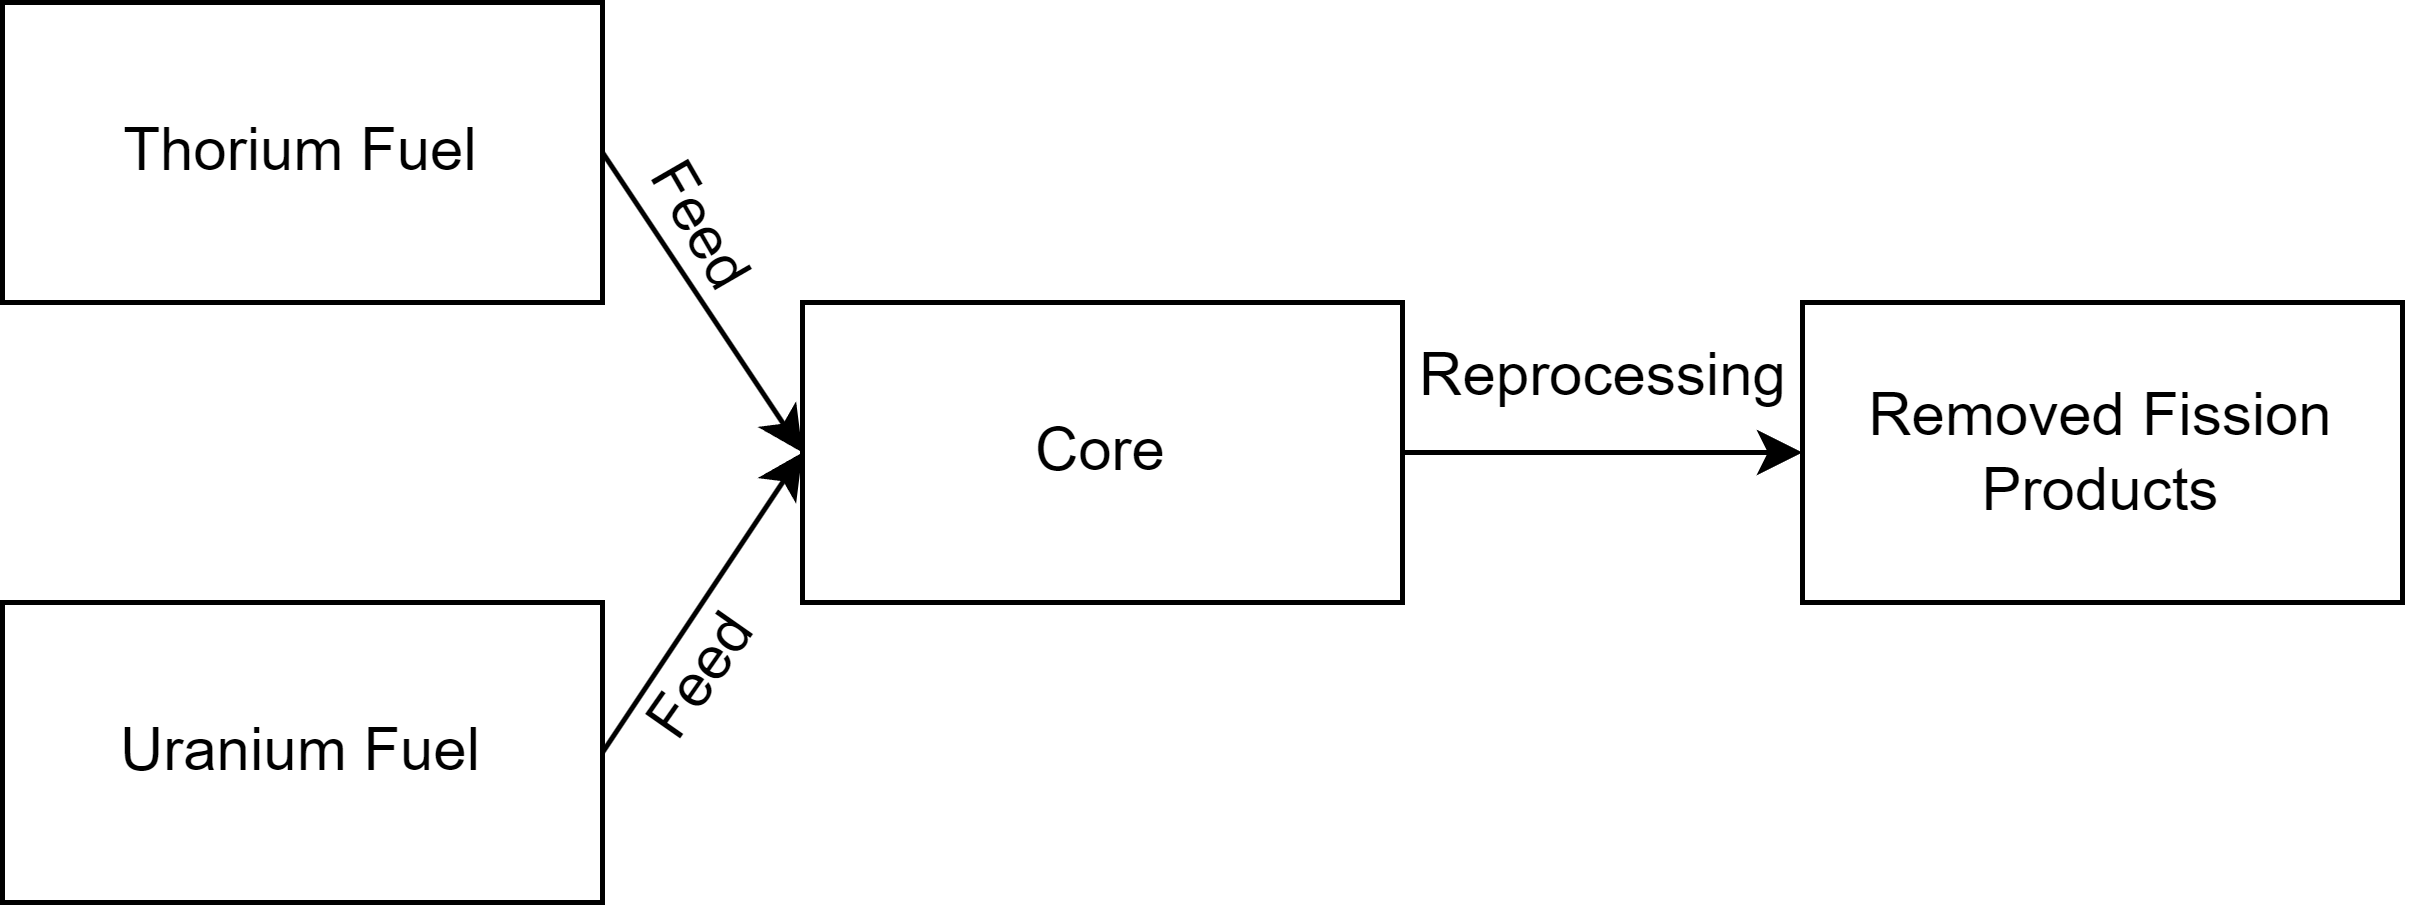
\includegraphics[scale=0.7]{images/sp-match-repr-scheme.png}
  \caption{Simplified reprocessing scheme based on mimicking SaltProc.}
   \label{fig:spmatchrepr}
\end{figure}

The second reprocessing scheme reflects the physical MSBR model, and instead uses a protactinium decay tank. From this tank, any bred uranium is continuously removed and sent back to the core, which is the intended design scheme for the MSBR \cite{robertson_conceptual_1971}. A simplified version of the phyiscally realistic uranium feed can be seen in Figure \ref{fig:nonspmatchrepr}.

\begin{figure}[H]
  \centering
  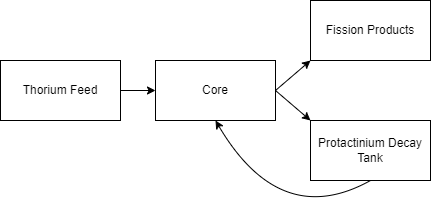
\includegraphics[scale=0.7]{images/phys-repr-scheme.png}
  \caption{Simplified reprocessing scheme based on the phyiscal MSBR processes.}
   \label{fig:nonspmatchrepr}
\end{figure}

Overall, it can be anticipated that the two methods will be approximately equal at steady state, since at that point the assumption by Rykhlevskii that the uranium input is the same as the protactinium output should be valid. However, there will be large differences for the first several months of operation, as the half life of protactinium-233 is on the order of one month, and the initial decrease in fissile material will impact reactor performance. This means that the uranium feed will take some time before it is providing a steady source of fissile material to the core.



%\chapter*{Appendix}
%Appendix.

\backmatter

\bibliographystyle{apalike}
\bibliography{bibliography}

\end{document}
\endinput
%%
%% End of file `thesis-ex.tex'.
